\chapter{Evaluation\label{cha:chapter6}}

In this chapter I will evaluate the different C2PA signing methods and present the benchmarks I put these through alongside their results and observations.

\section{Test Environment\label{sec:testenvir}}

I ran the benchmarks on the Work Laptop 2 shown in \Cref{tab:env}. In total I ran two\todo{num benchmarks} benchmarks to measure the performance of the original Merkle Tree, optimized Merkle Tree and Rolling Hash approaches.

For these benchmarks I prepared 100 fragments for four different media representations: one audio track and three video tracks with vastly different file sizes. I chose to use only one audio quality, because from experience it is not that common to have multiple audio quality, if there are multiple qualities they are usually different languages with the same encoding. The audio setting I use are the same that are found in the default audio settings of the Producer, shown in \Cref{list:audio}, with an average file size of \texttt{31 kilobyte}. The three video tracks represent a low, mid and high encoding quality each. The settings are taken from the default video settings of the Producer, shown in \Cref{list:video}. The low options is represented by the \texttt{240p} setting with an average file size of \texttt{64 kilobyte}, the mid option is taken from the \texttt{720p} (HD) setting with an average file size of \texttt{467 kilobyte} and the high option is the \texttt{2160p} (4k) setting with an average file size of \texttt{3,752 kilobyte}. All file sizes are shown in \Cref{fig:file-size}.

\begin{figure}[t]
    \centering
    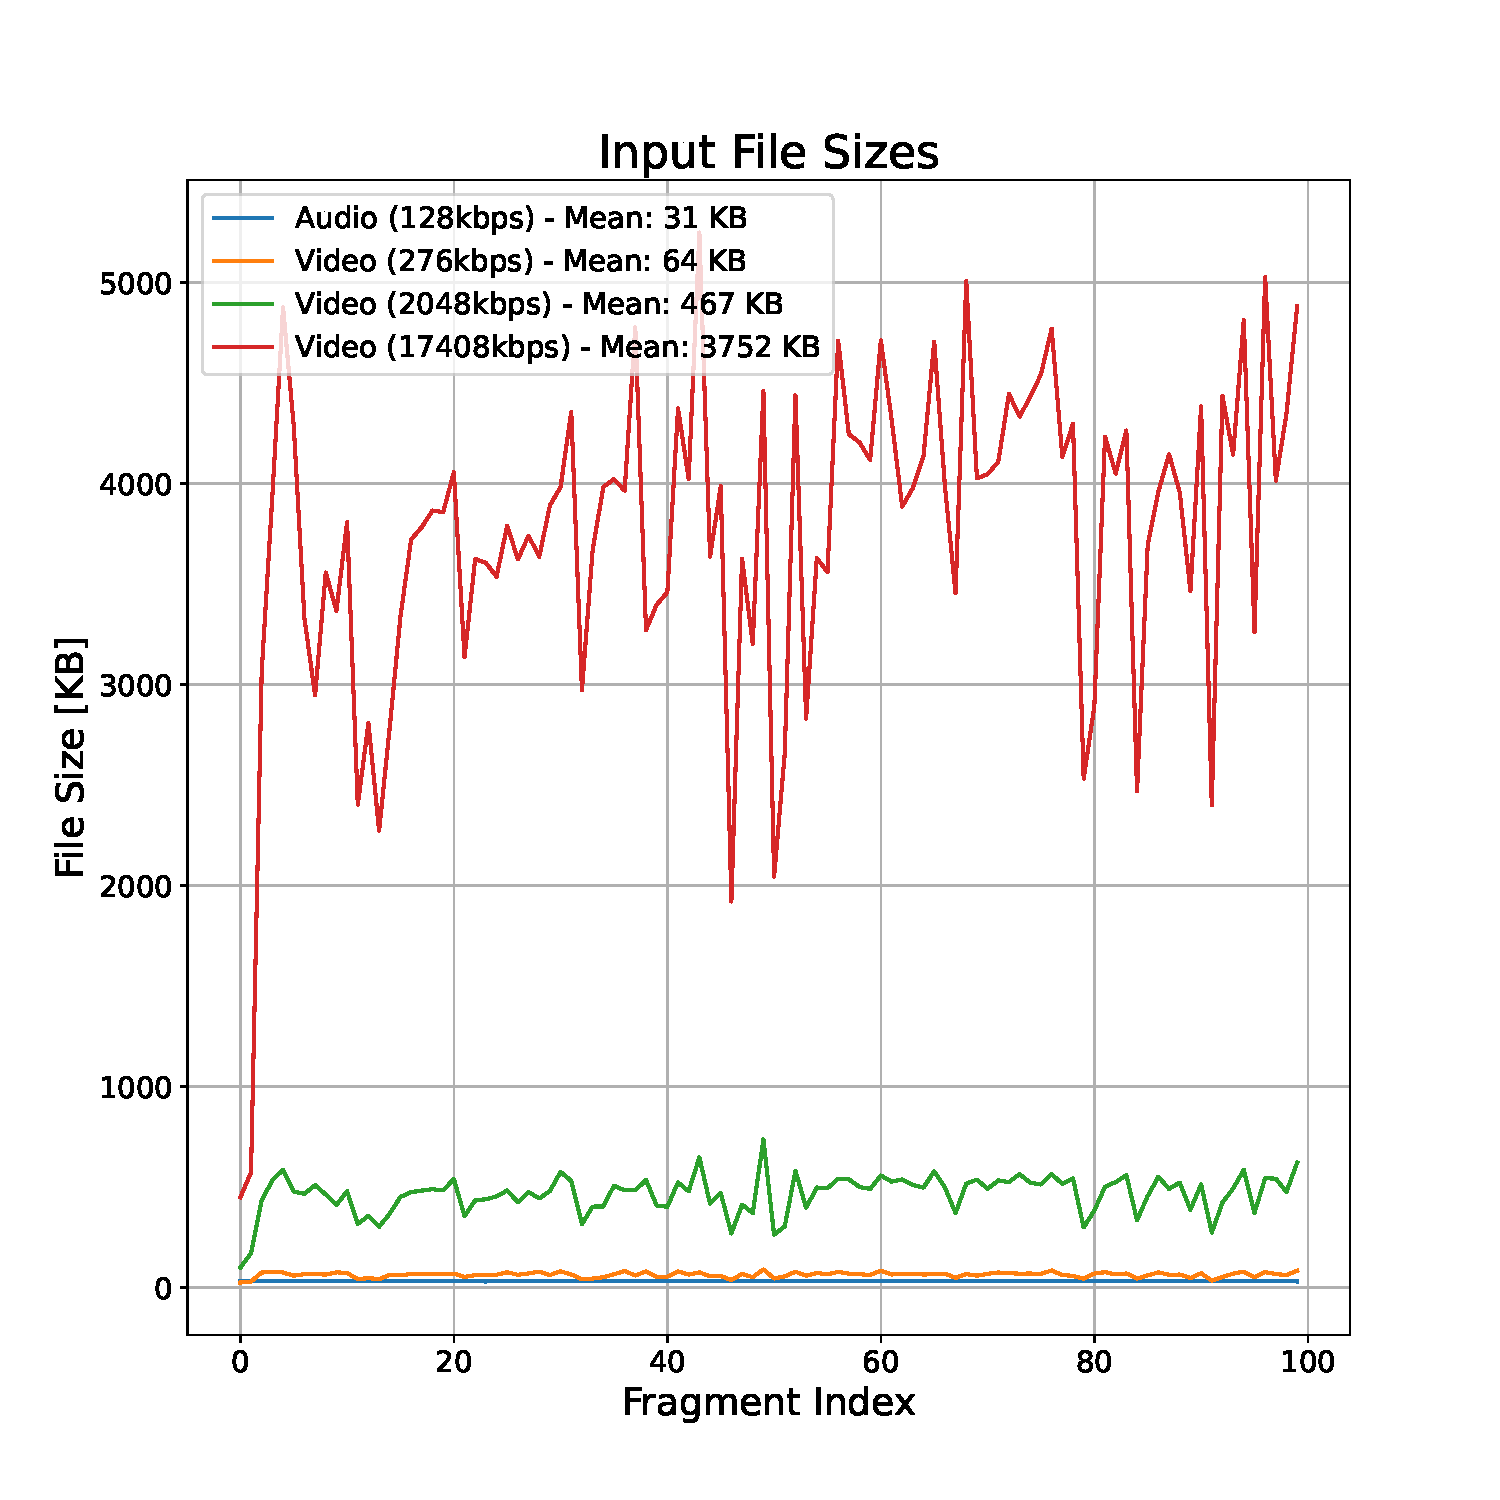
\includegraphics[width=0.75\linewidth]{plots/input-sizes.pdf}
    \caption{Input File Sizes}
    \label{fig:file-size}
\end{figure}

\subsection{Signing Duration}

In this benchmark I measured how long the entire signing function runs for to sign a live stream with up to 100 fragments. For this benchmark I loop through all available representations then for each signing method I iterate from 1 to 100 and sign the live stream at each index in accordance to the method. For the Rolling Hash signing this means that only the current fragments of that index is being signed. For the case of the optimized Merkle Tree approach I provide the signing function with the paths too all fragments to to the current index, but only the up to window size (eight) number of fragments are actually signed and for the original Merkle Tree every single fragment is being signed.

The lower the time it takes to sign the newly created fragments the less the impact on the streaming latency is, lower is better.

The time measuring can be described with the pseudo code from \Cref{alg:time-measure}. Essentially, I take a timestamp right before signing the fragments and right after the signing I take a second timestamp and the difference between the two timestamps is the time it took to sign the fragments. Then I save this value in a data structure in relation to the fragment index and representation the fragment belongs to.

\begin{algorithm}[H]
    \begin{algorithmic}[1]
        \State $now \gets Time.now()$
        \State sign\_fragments()
        \State $time \gets Time.since(now)$        
    \end{algorithmic}
    \caption{Duration Measuring Method}
    \label{alg:time-measure}
\end{algorithm}

In total I ran this benchmark ten times and averaged all results.

\subsection{Data Upload Size Required}

For this benchmark I looked at how much data has to be published to the CDN after each fragment has been signed. I measured this by simply adding up the file sizes of all the files that were effected the signing of the current fragments, which would subsequently needed to be uploaded to the CDN. In case of Rolling Hash that is only the initialization fragment and the fragment at the current index. For the optimized Merkle Tree approach that is the initialization fragment and all fragments of the current Merkle Tree, which are up to eight fragments with my configuration and again all fragments for the original Merkle Tree signing.

Since this benchmark is merely adding up file sizes I ran this one in conjunction with the previous duration benchmark, so I don't have to sign everything multiple times for each benchmark.

In this benchmark a lower upload size equals to less overhead on the network and a better caching situation for the CDN, again lower is better.

\section{Performance Measurements\label{sec:performance}}

In this section I will present the results of the above described benchmarks and give my evaluation and observations about them.

\subsection{Signing Duration}

I have split the data plots into two comparisons. One comparing each signing method in relation to the different representations, shown in \Cref{fig:sign-dur1} and the other comparing the signing method to each other per representation, shown in \Cref{fig:sign-dur2}.

\todo{describe results}

\begin{figure}
    \centering
    \subfloat[Original Merkle Tree]{
        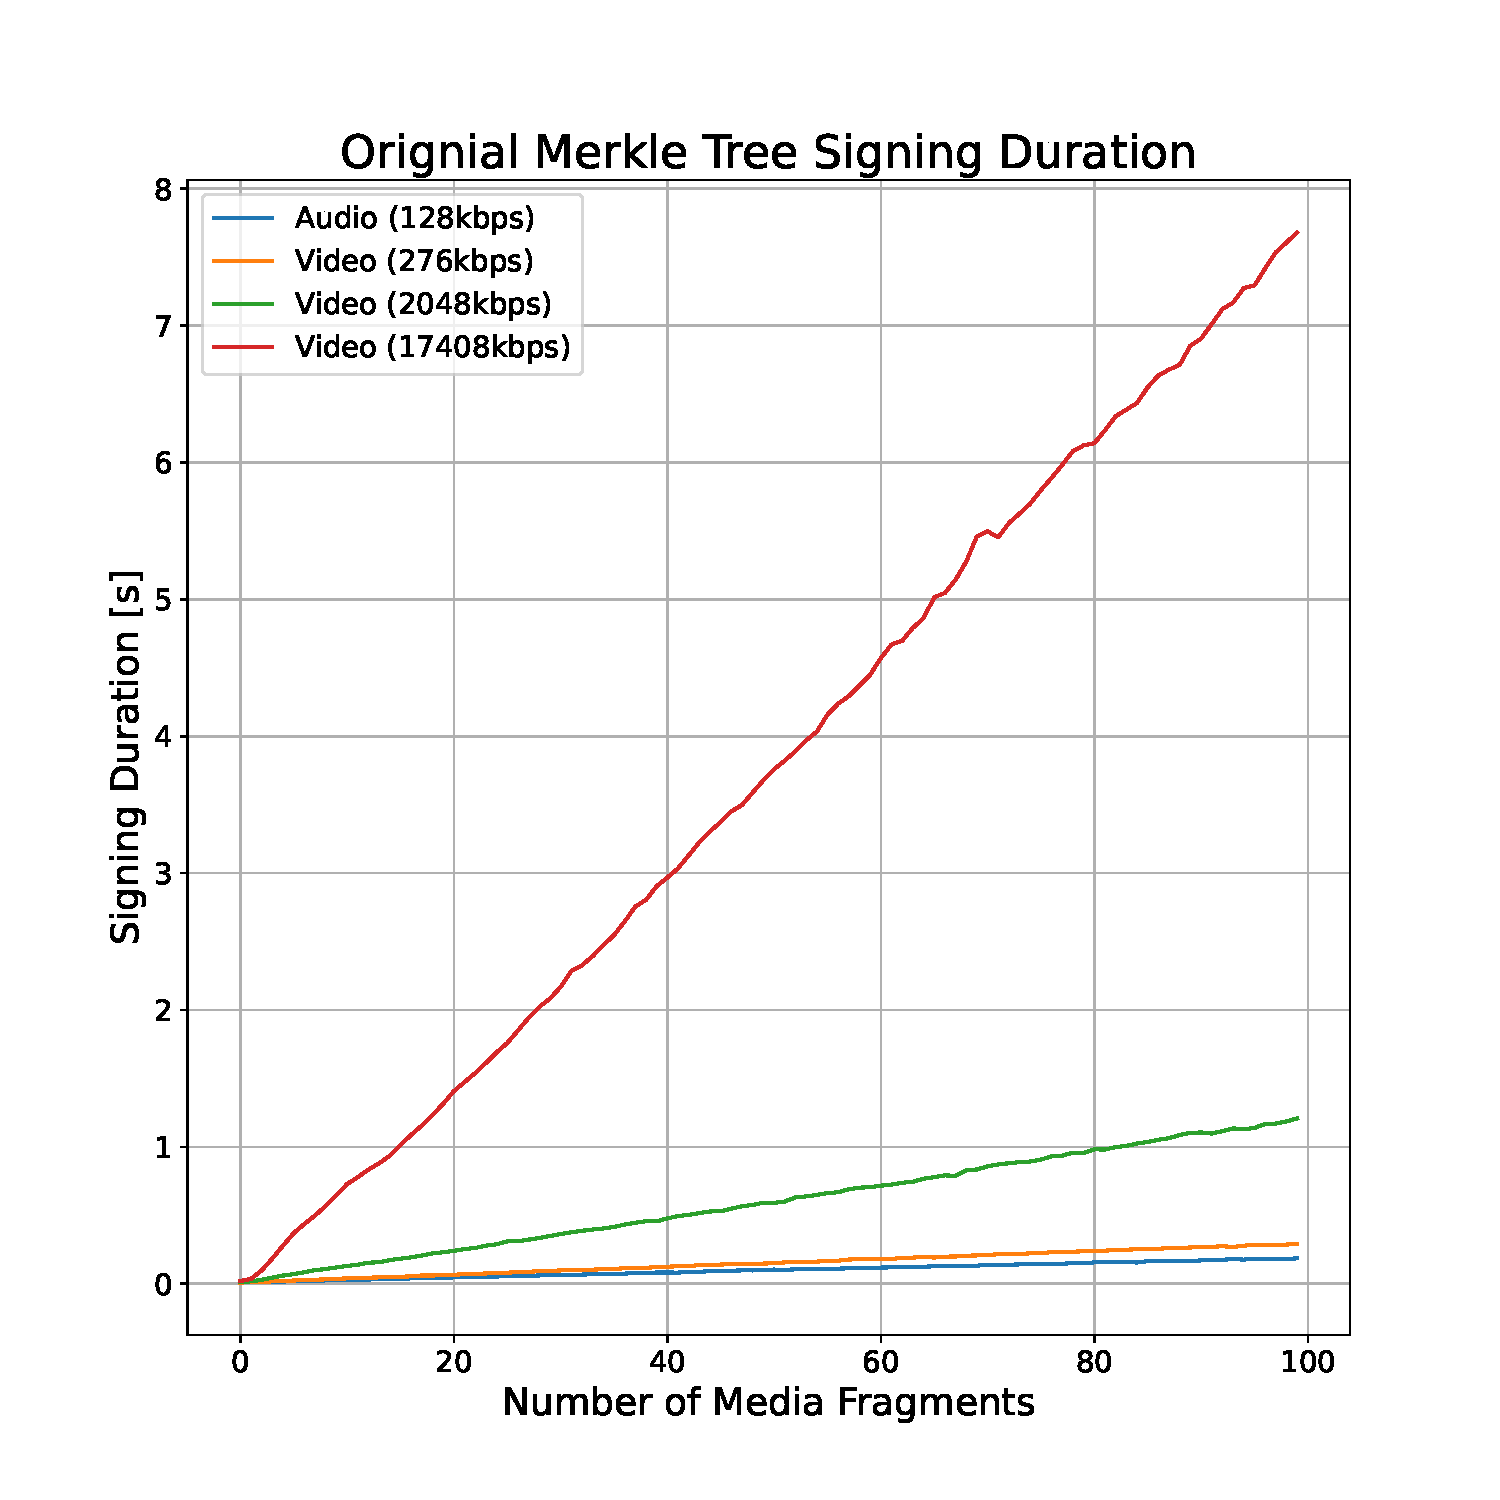
\includegraphics[width=0.49\linewidth]{plots/time-orignial-merkle-tree.pdf}
        \label{fig:sign-dur1-og}
    }
    \subfloat[Optimized Merkle Tree]{
        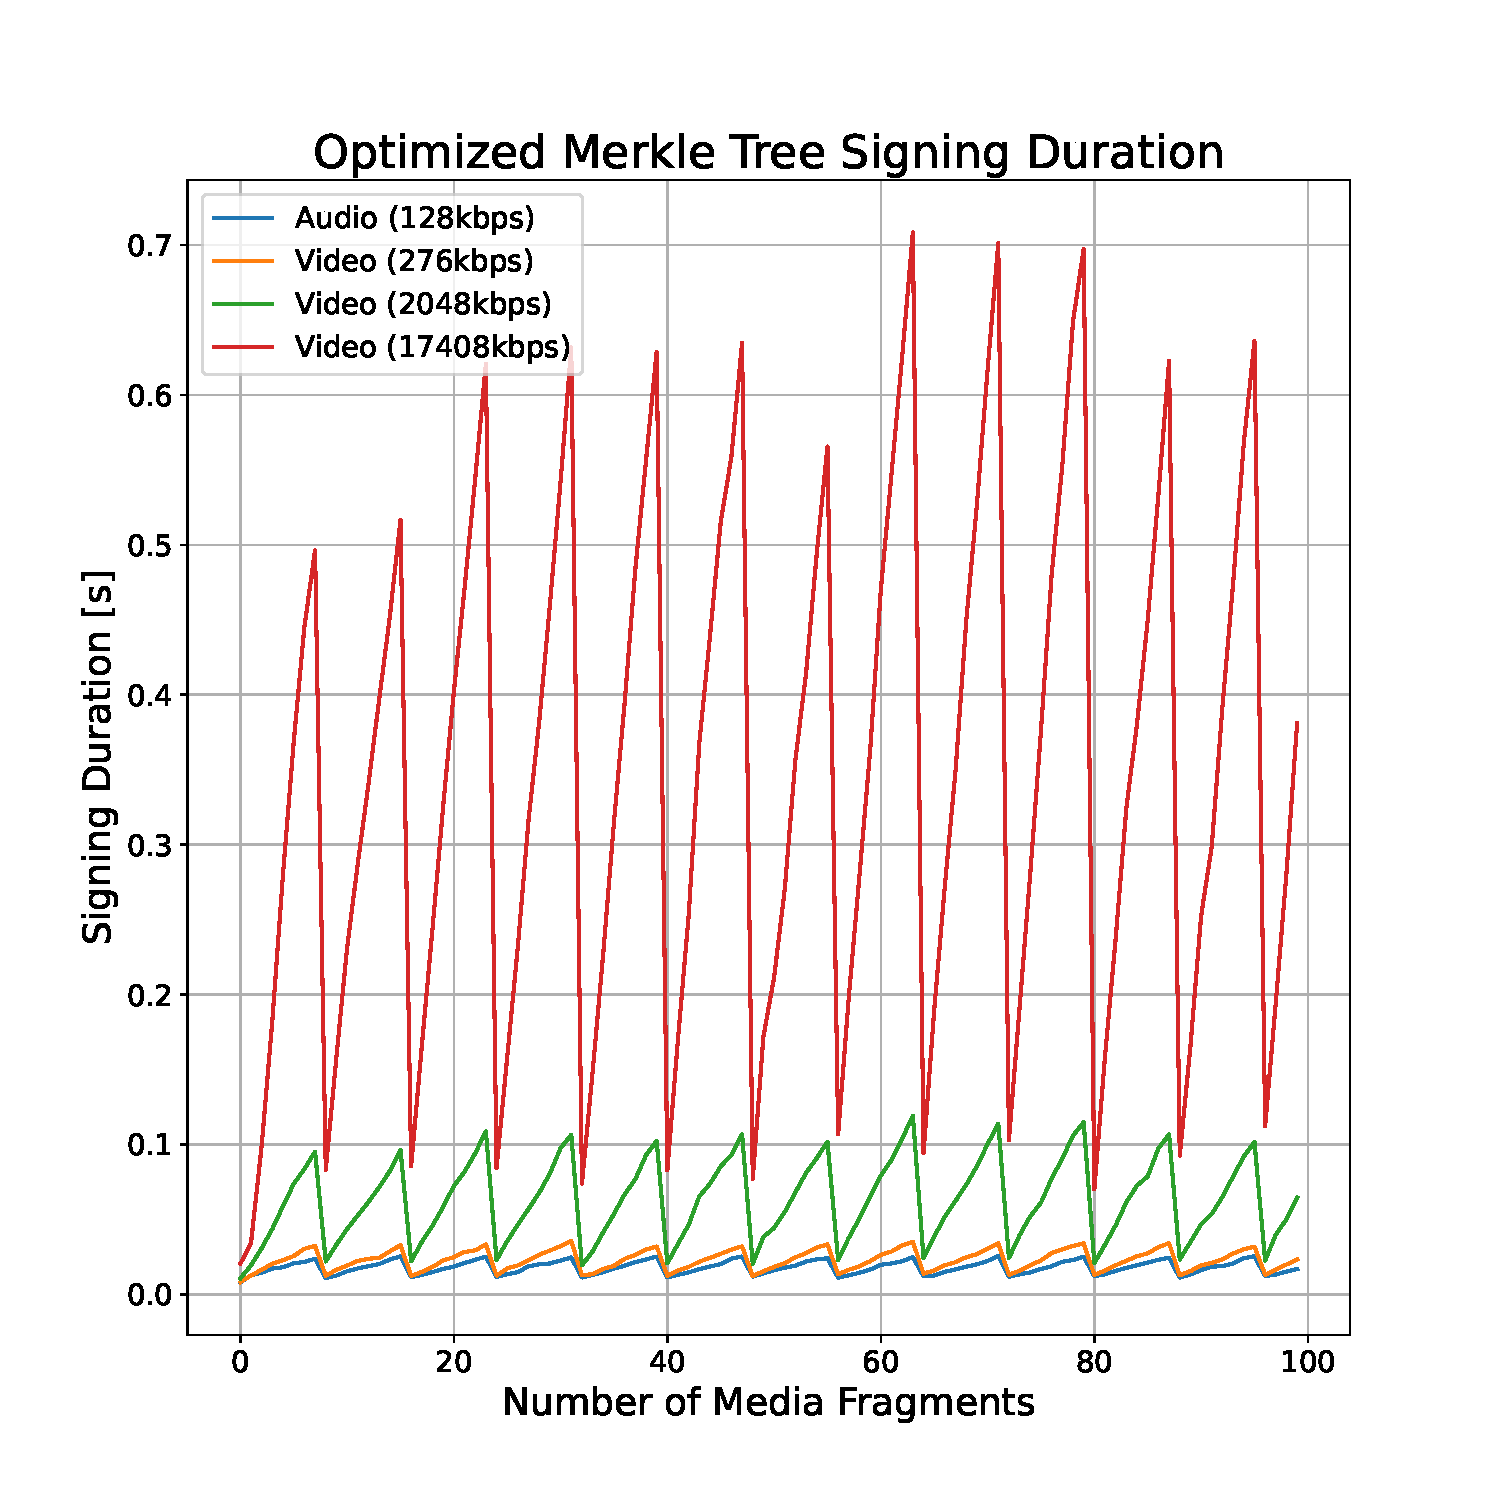
\includegraphics[width=0.49\linewidth]{plots/time-optimized-merkle-tree.pdf}
        \label{fig:sign-dur1-opt}
    } \\
    \subfloat[Rolling Hash]{
        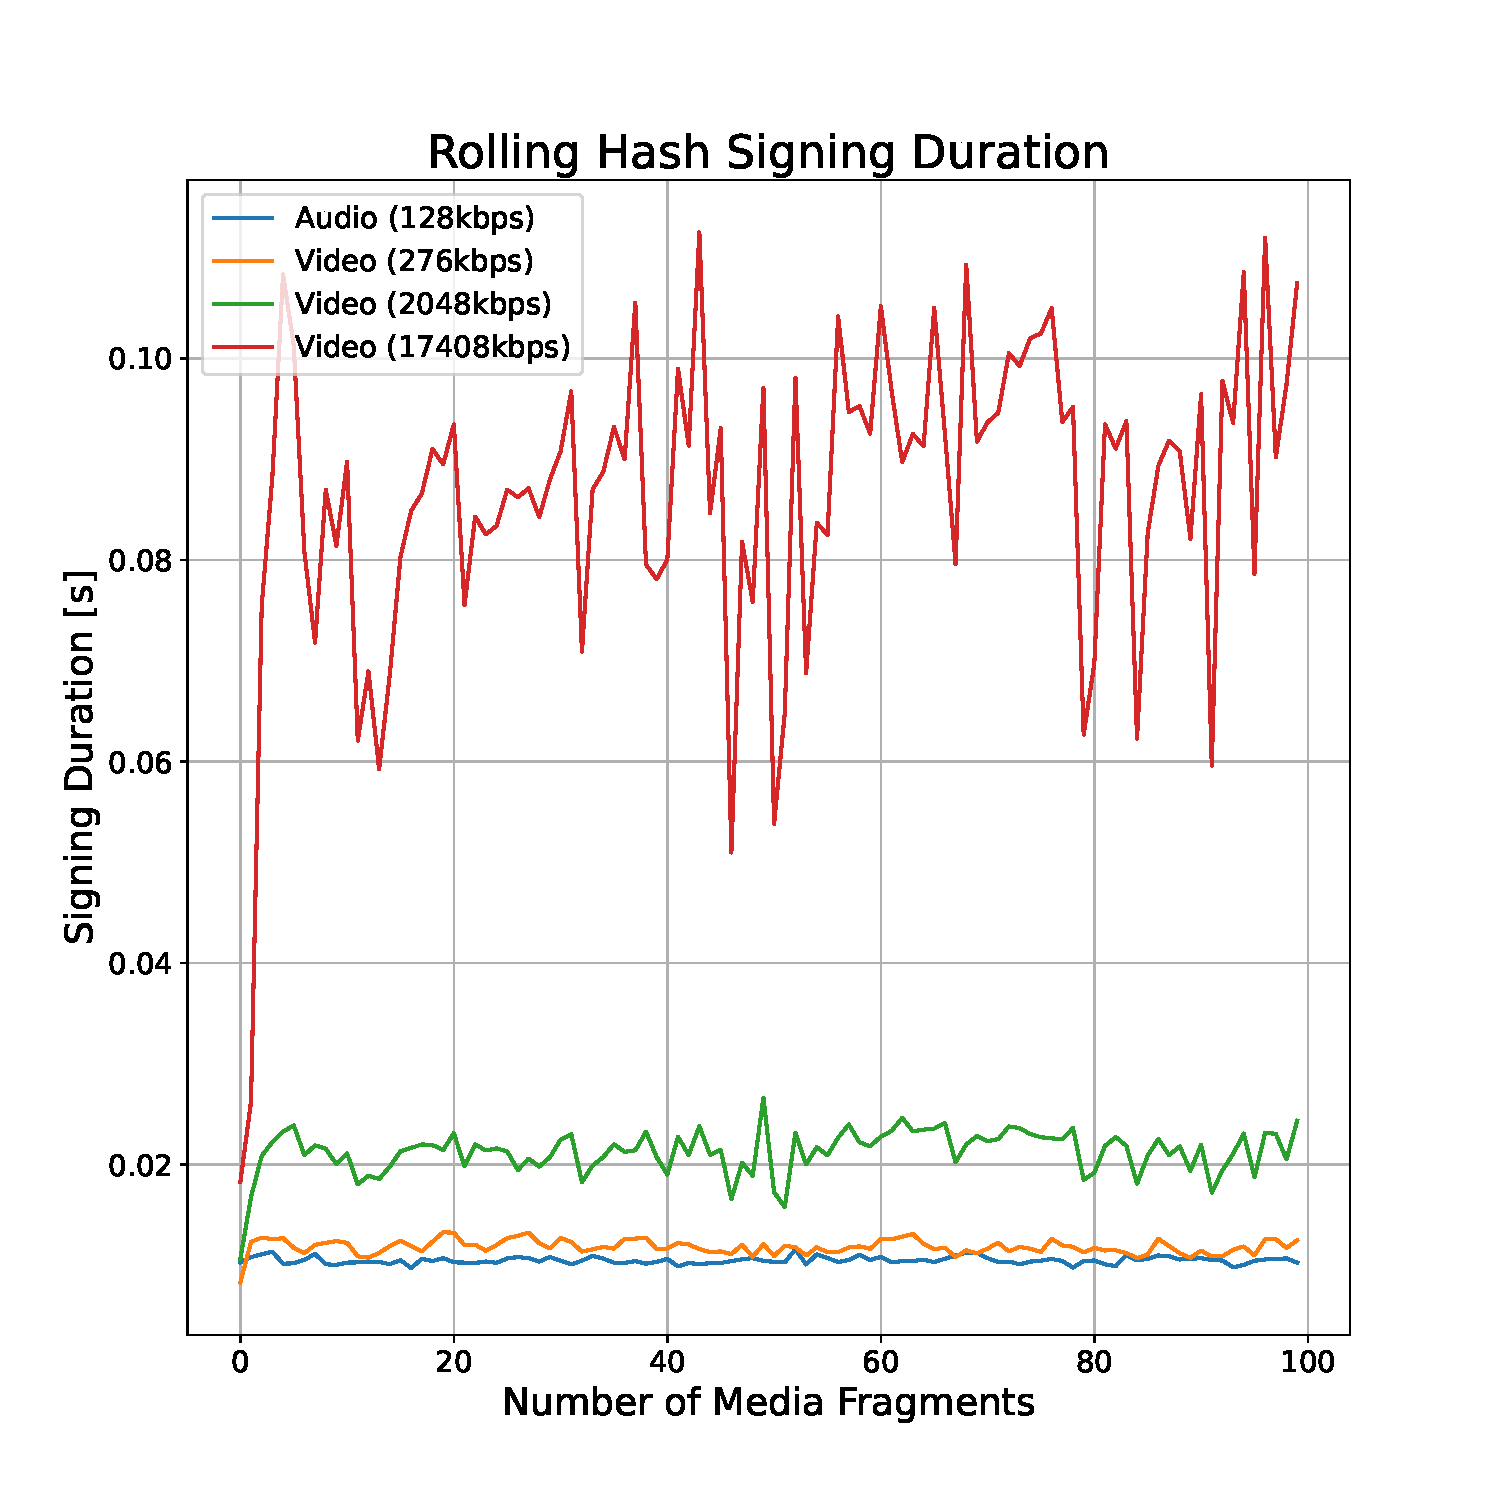
\includegraphics[width=0.49\linewidth]{plots/time-rolling-hash.pdf}
        \label{fig:sign-dur1-rh}
    }
    \caption{Signing Duration Results}
    \label{fig:sign-dur1}
\end{figure}

\begin{figure}
    \centering
    \subfloat[Audio (128kbps)]{
        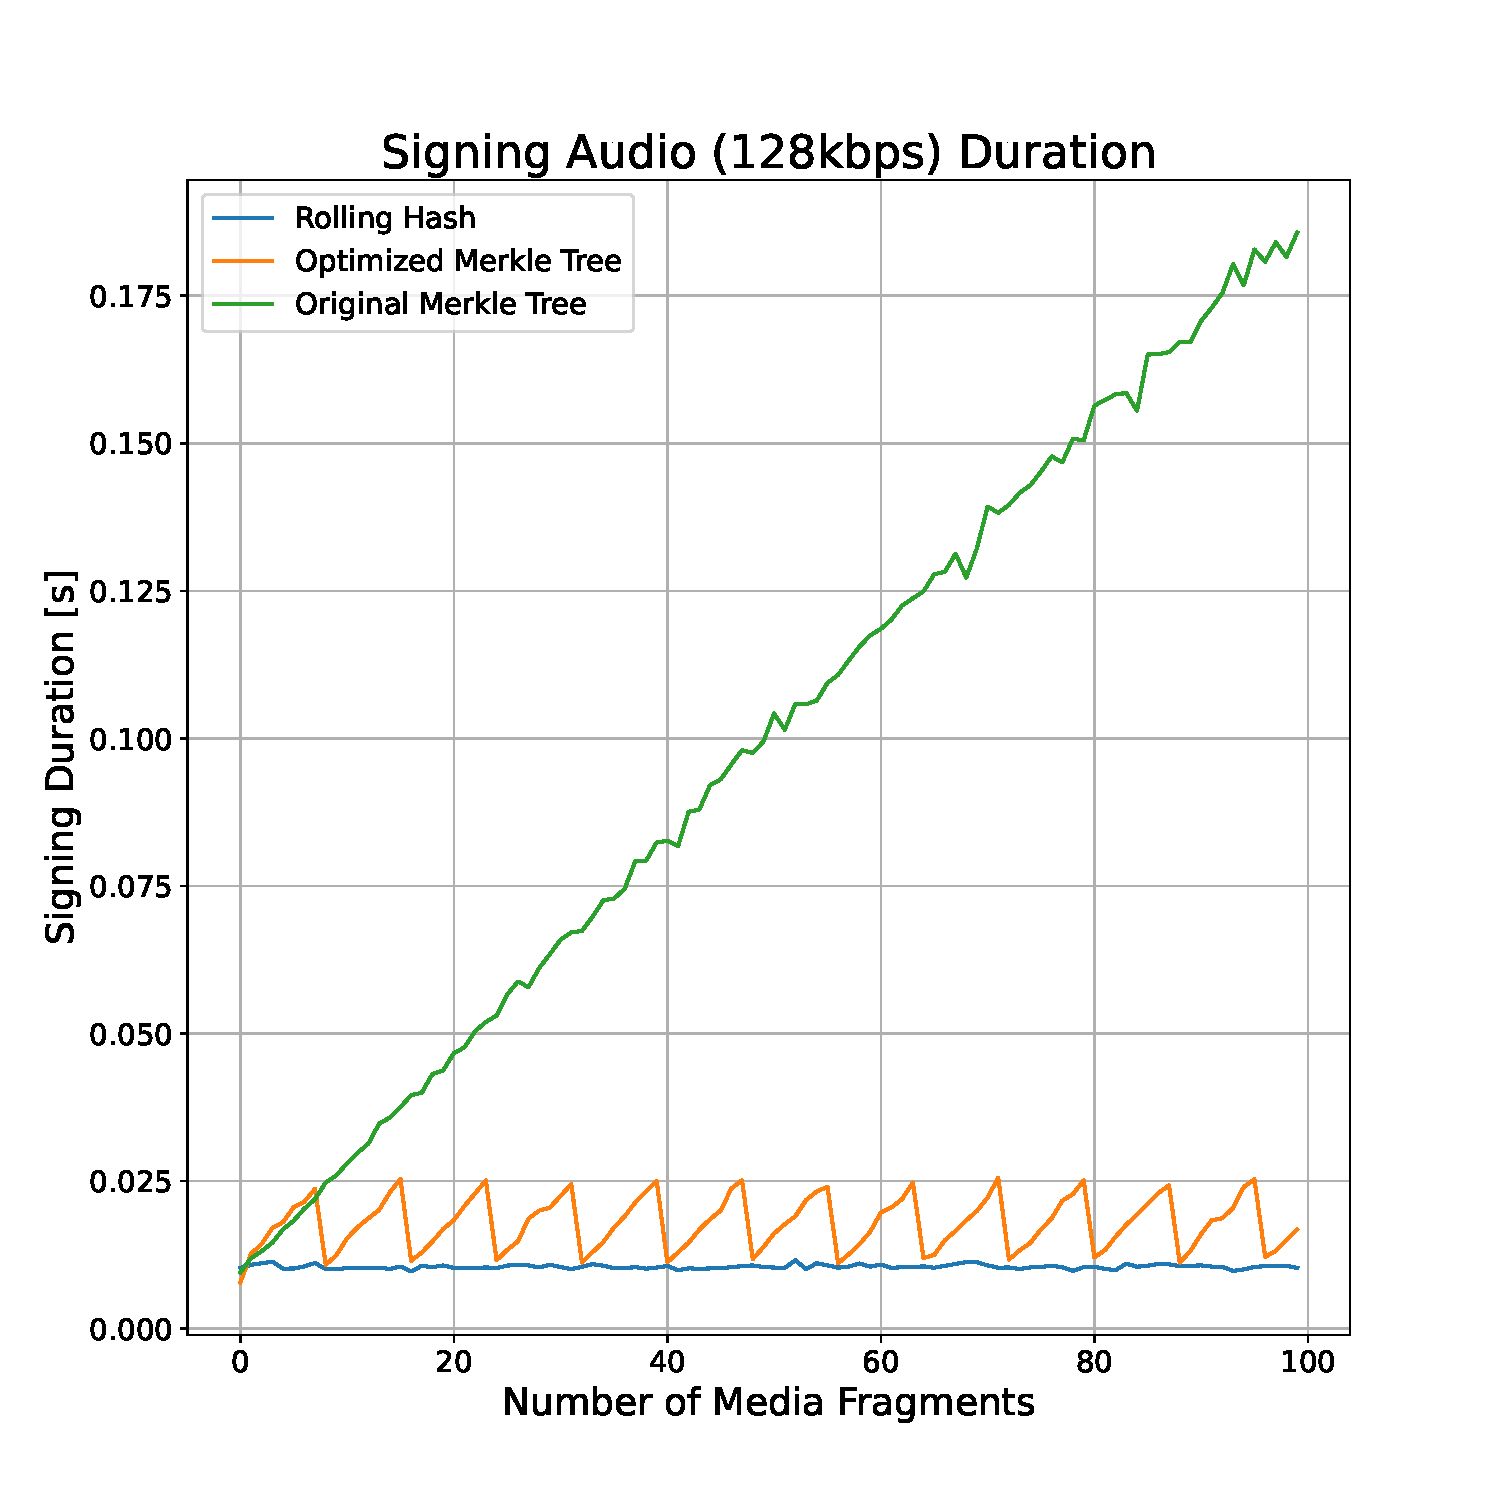
\includegraphics[width=0.49\linewidth]{plots/compare-time-Audio-(128kbps).pdf}
        \label{fig:sign-dur2-audio}
    }
    \subfloat[Video (276kbps)]{
        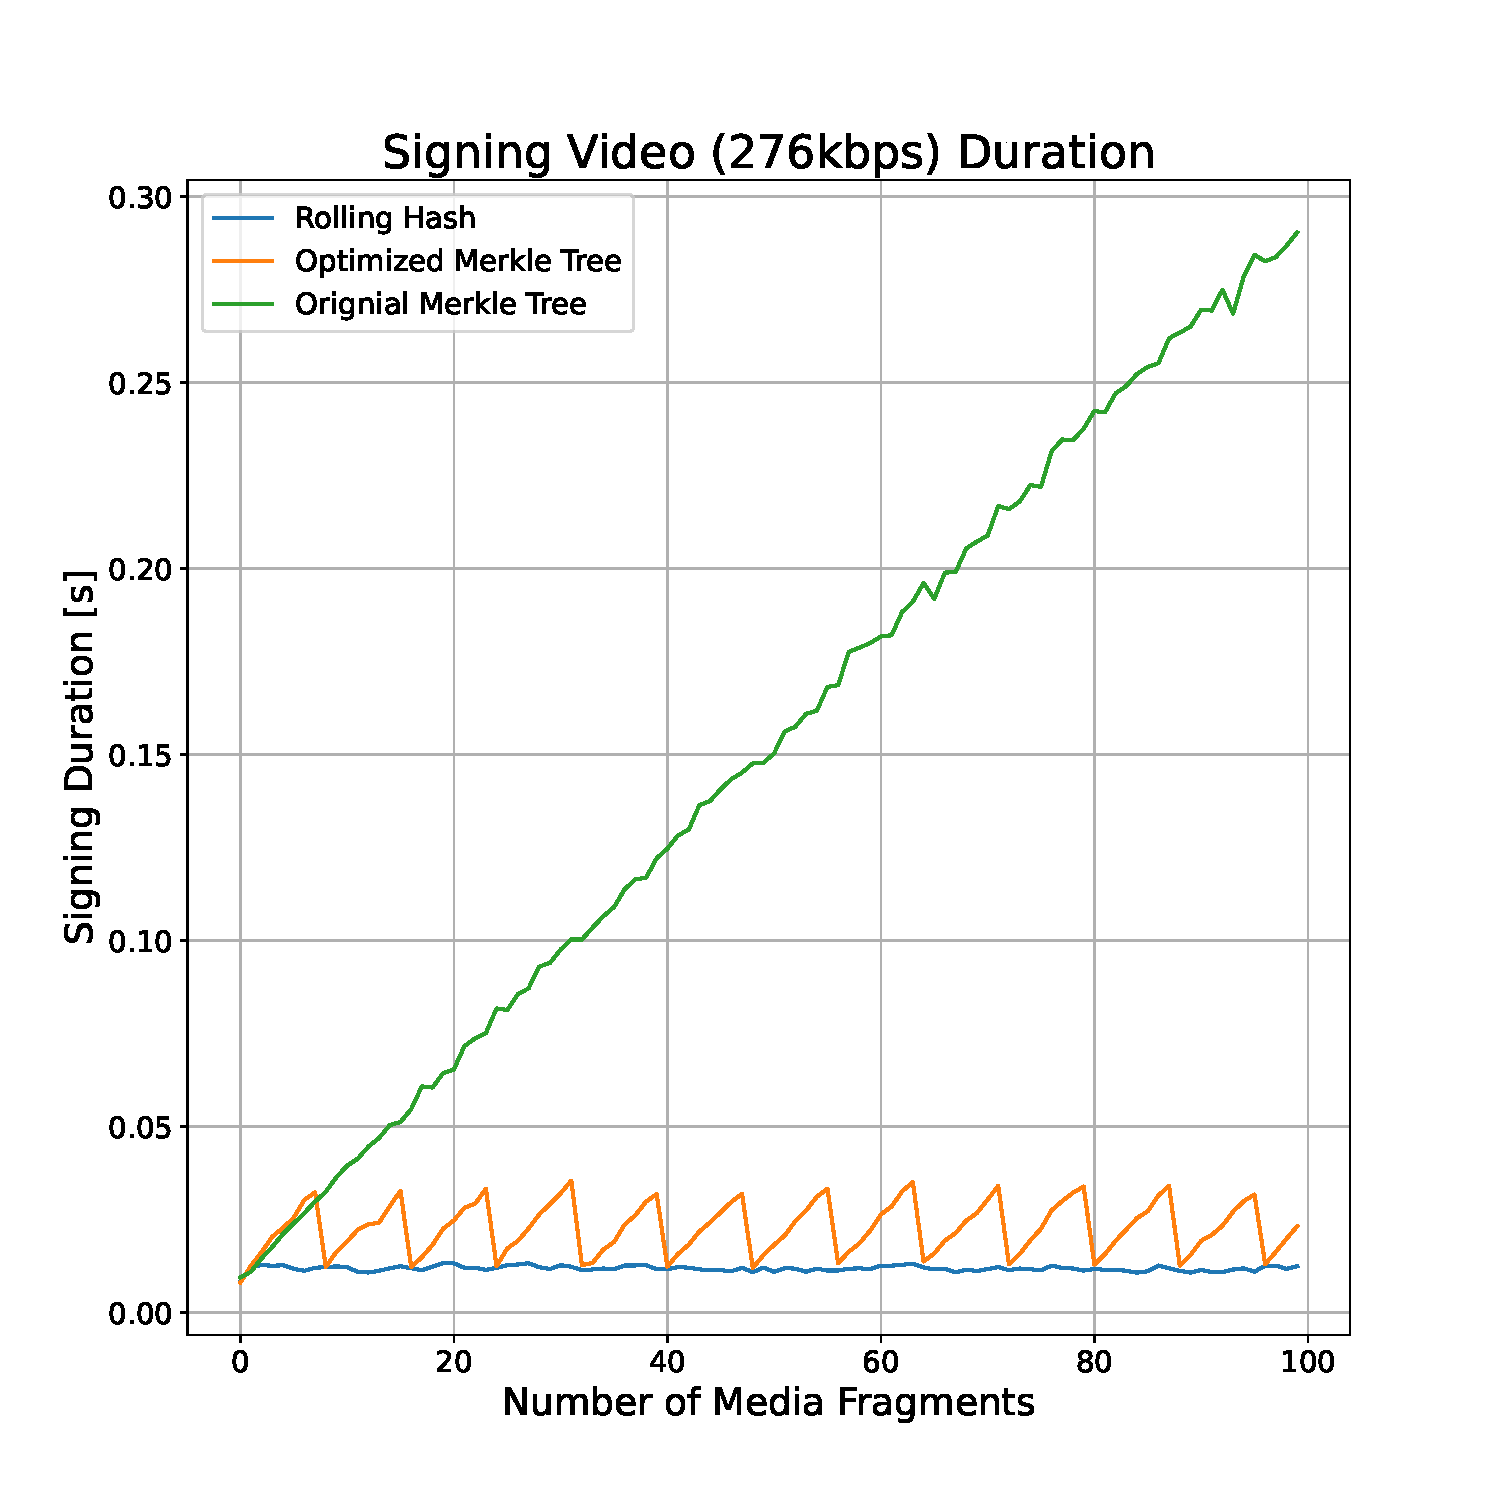
\includegraphics[width=0.49\linewidth]{plots/compare-time-Video-(276kbps).pdf}
        \label{fig:sign-dur2-video1}
    } \\
    \subfloat[Video (2,048kbps)]{
        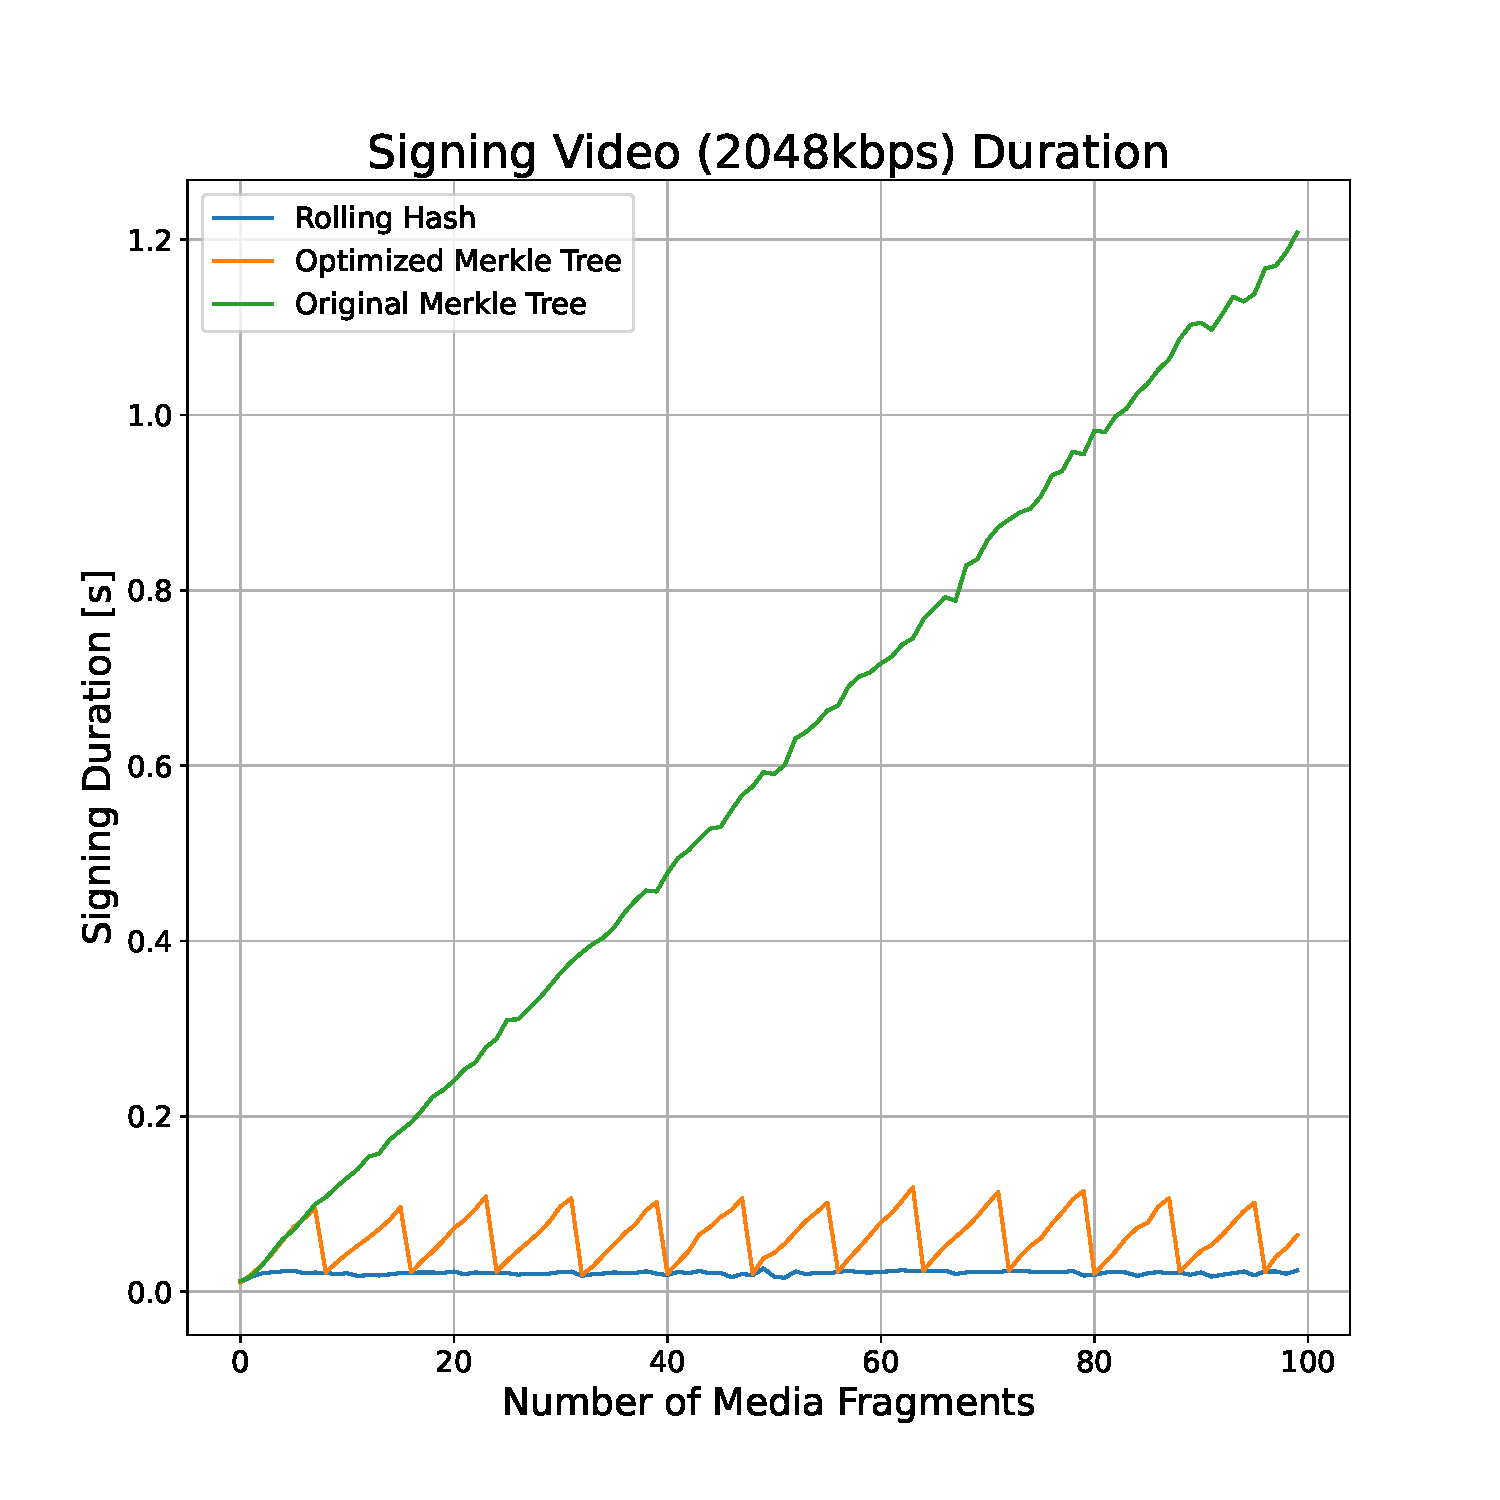
\includegraphics[width=0.49\linewidth]{plots/compare-time-Video-(2048kbps).pdf}
        \label{fig:sign-dur2-video2}
    }
    \subfloat[Video (17,408kbps)]{
        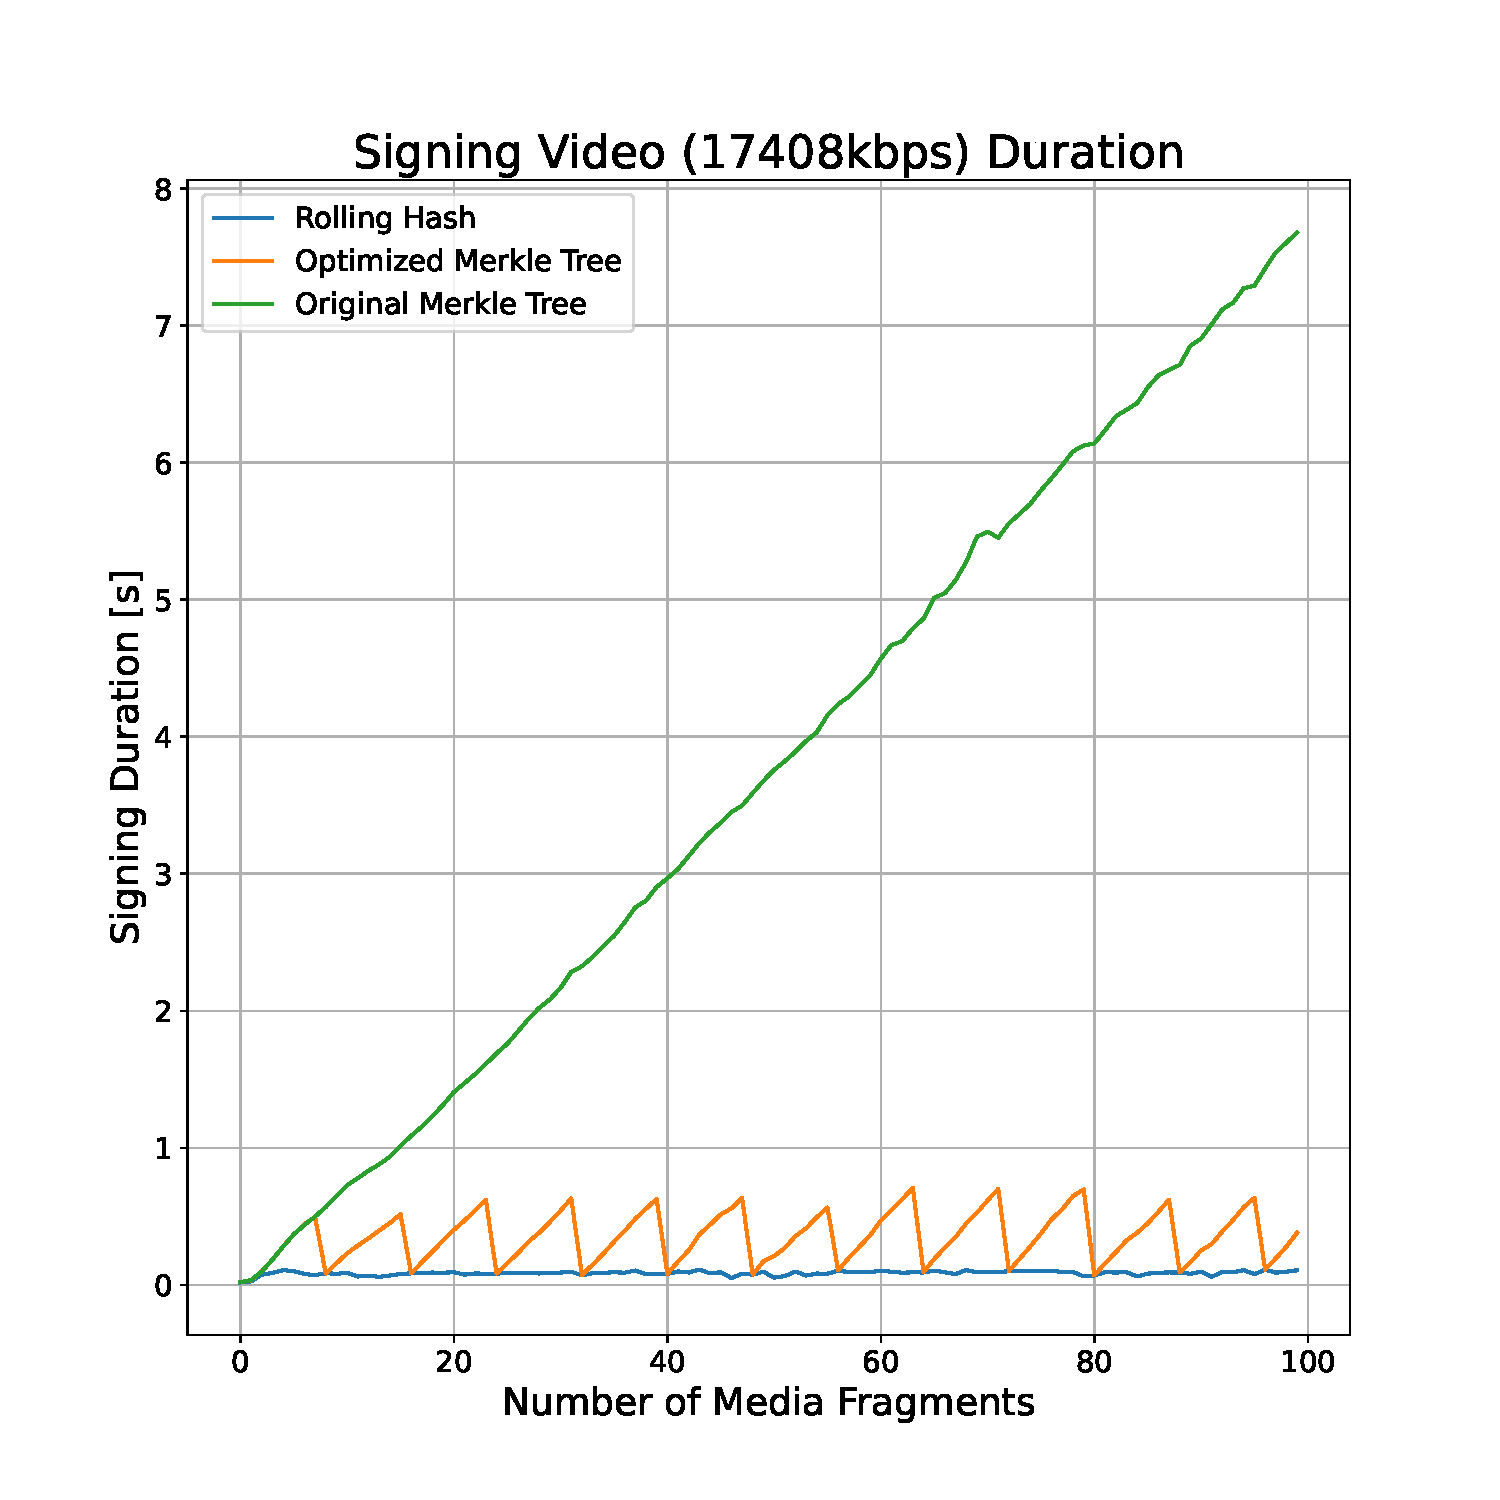
\includegraphics[width=0.49\linewidth]{plots/compare-time-Video-(17408kbps).pdf}
        \label{fig:sign-dur2-video3}
    }
    \caption{Signing Duration Results}
    \label{fig:sign-dur2}
\end{figure}

\subsection{Data Upload Size Required}

For this benchmark I have split the data plots into the same comparisons as before: comparing each signing method in relation to the different representations are shown in \Cref{fig:upload1} and the signing methods compared to each other per representation are shown in \Cref{fig:upload2}.

\todo{describe results}

\begin{figure}
    \centering
    \subfloat[Original Merkle Tree]{
        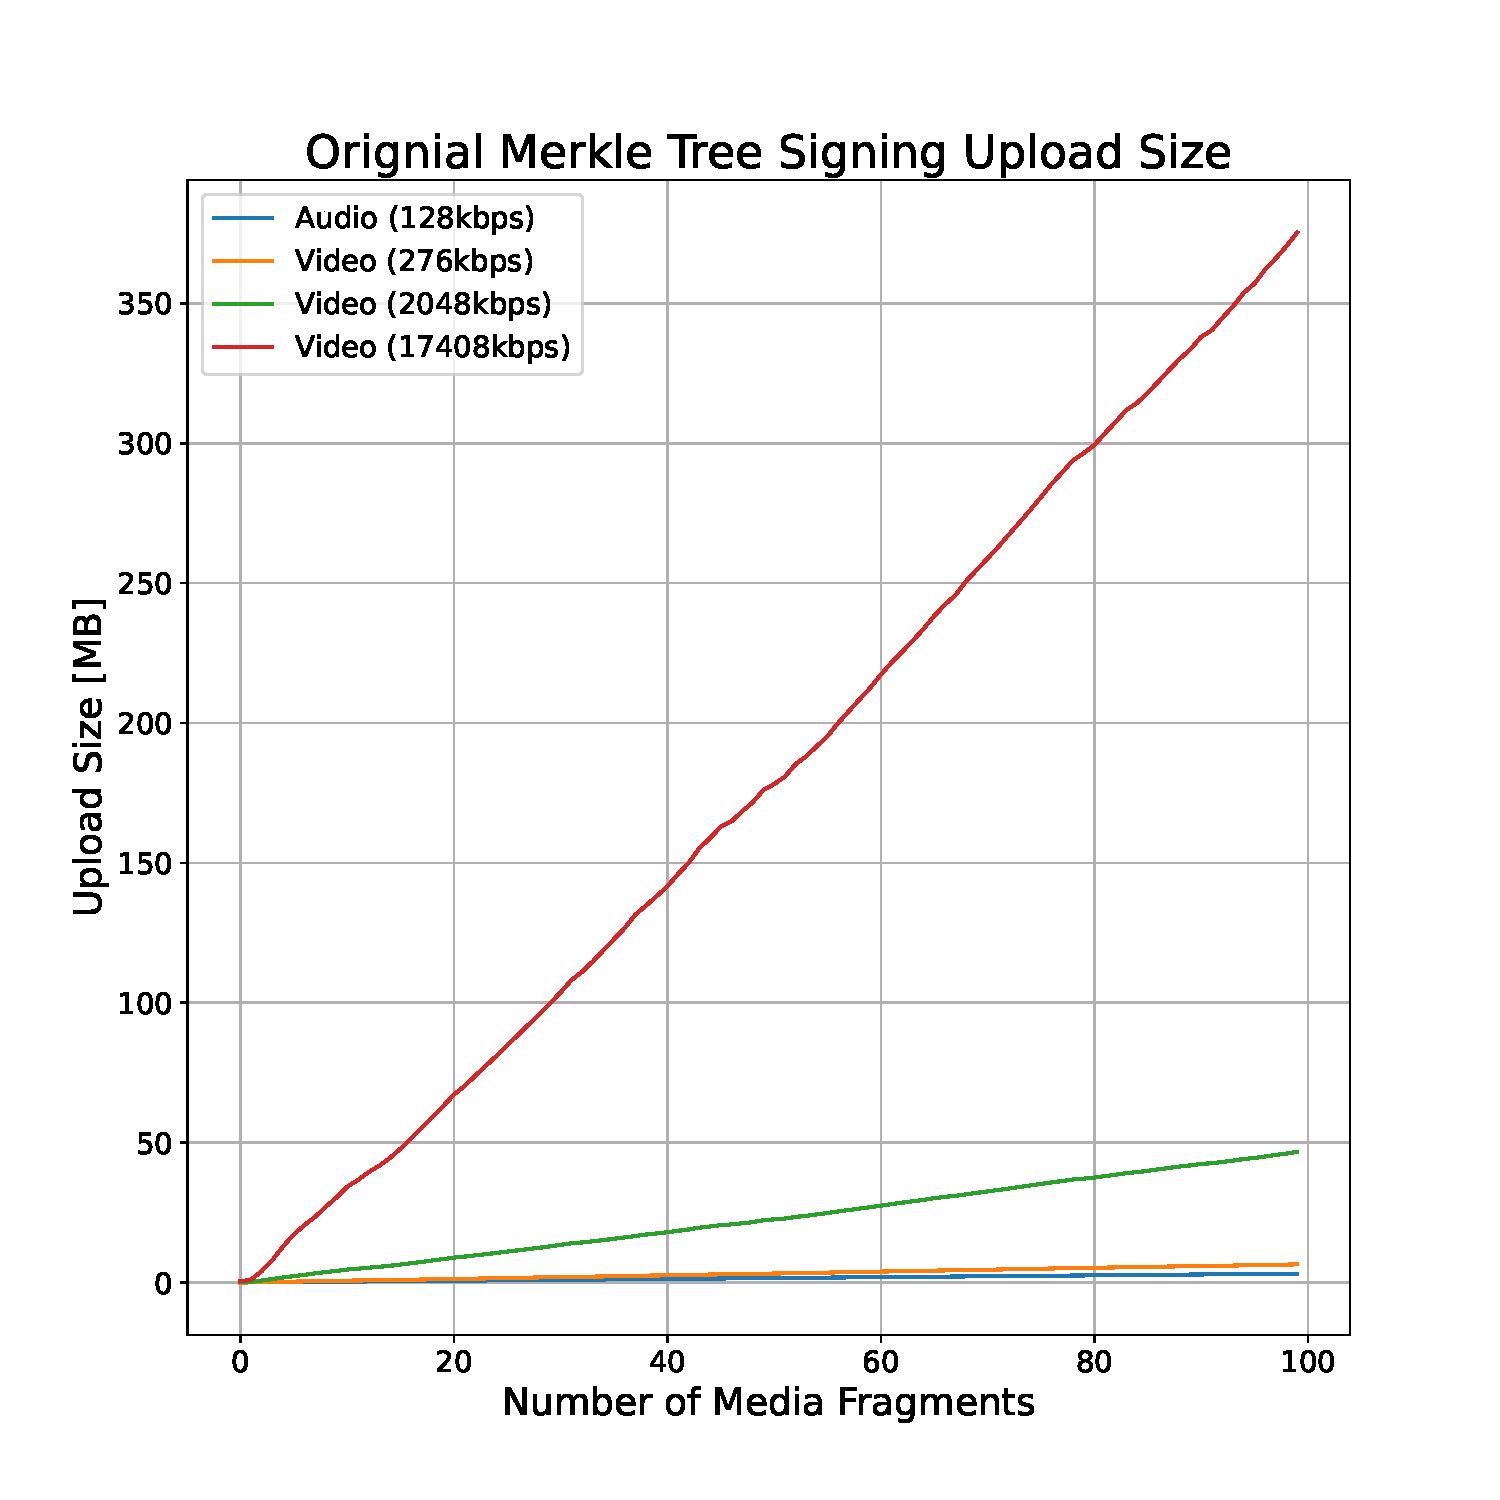
\includegraphics[width=0.49\linewidth]{plots/upload-orignial-merkle-tree.pdf}
        \label{fig:upload1-og}
    }
    \subfloat[Optimized Merkle Tree]{
        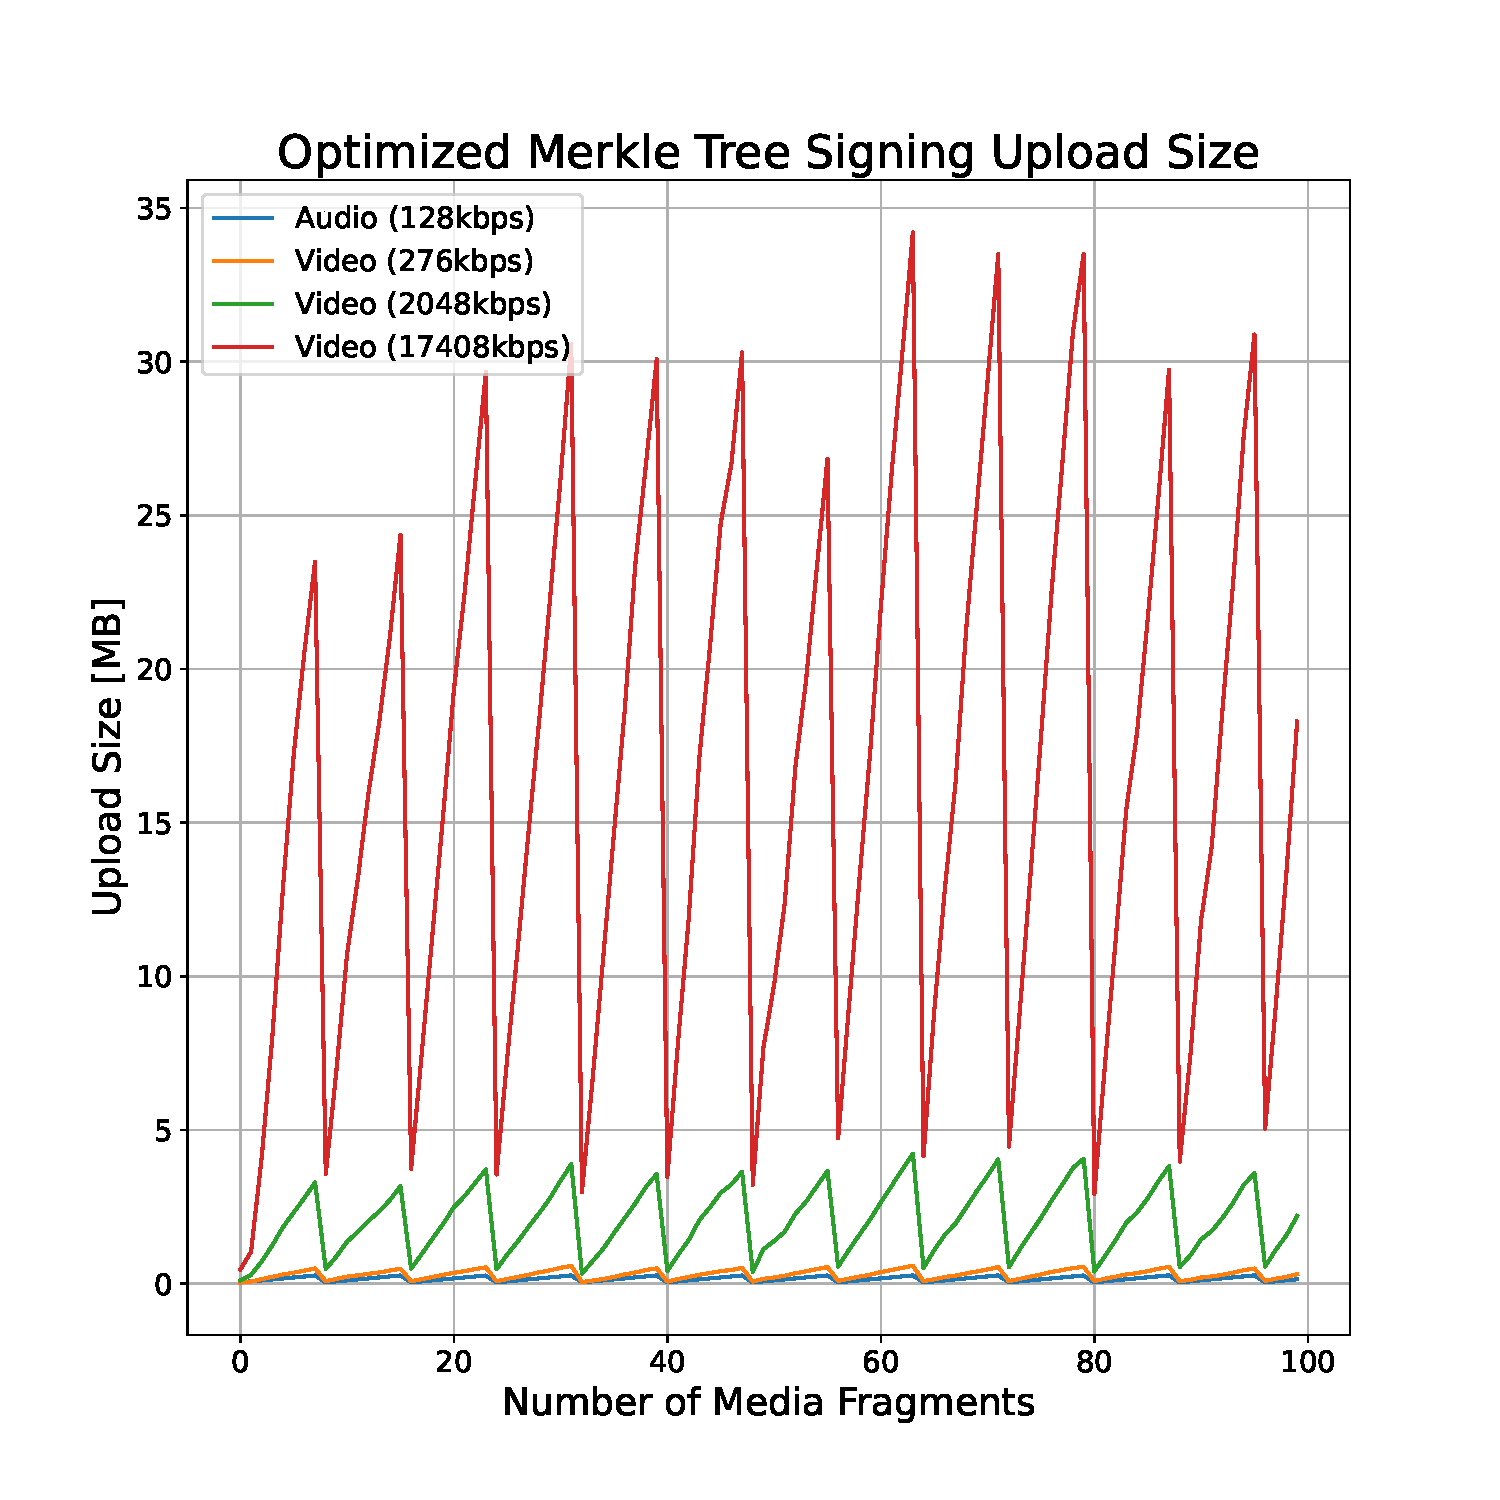
\includegraphics[width=0.49\linewidth]{plots/upload-optimized-merkle-tree.pdf}
        \label{fig:upload1-opt}
    } \\
    \subfloat[Rolling Hash]{
        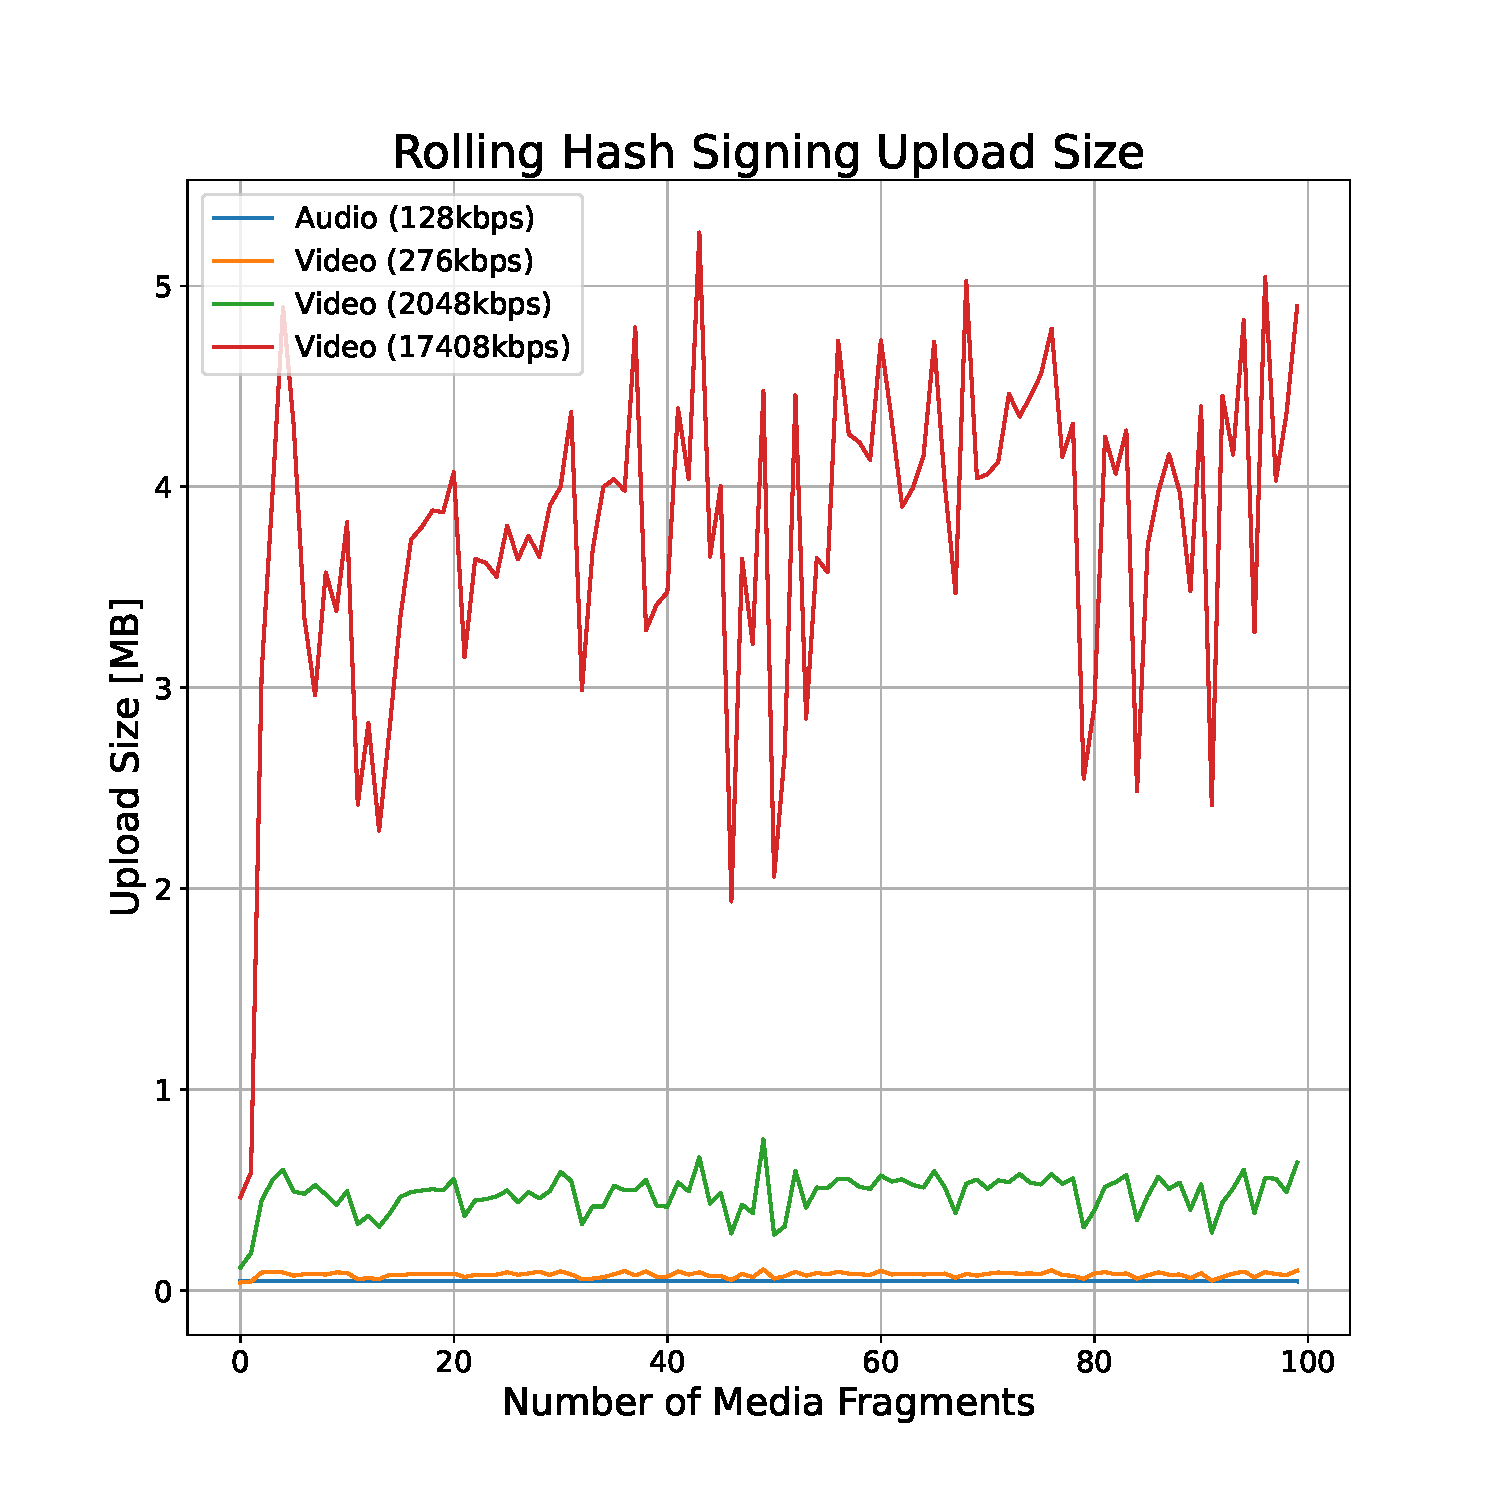
\includegraphics[width=0.49\linewidth]{plots/upload-rolling-hash.pdf}
        \label{fig:upload1-rh}
    }
    \caption{Upload Size Results}
    \label{fig:upload1}
\end{figure}

\begin{figure}
    \centering
    \subfloat[Audio (128kbps)]{
        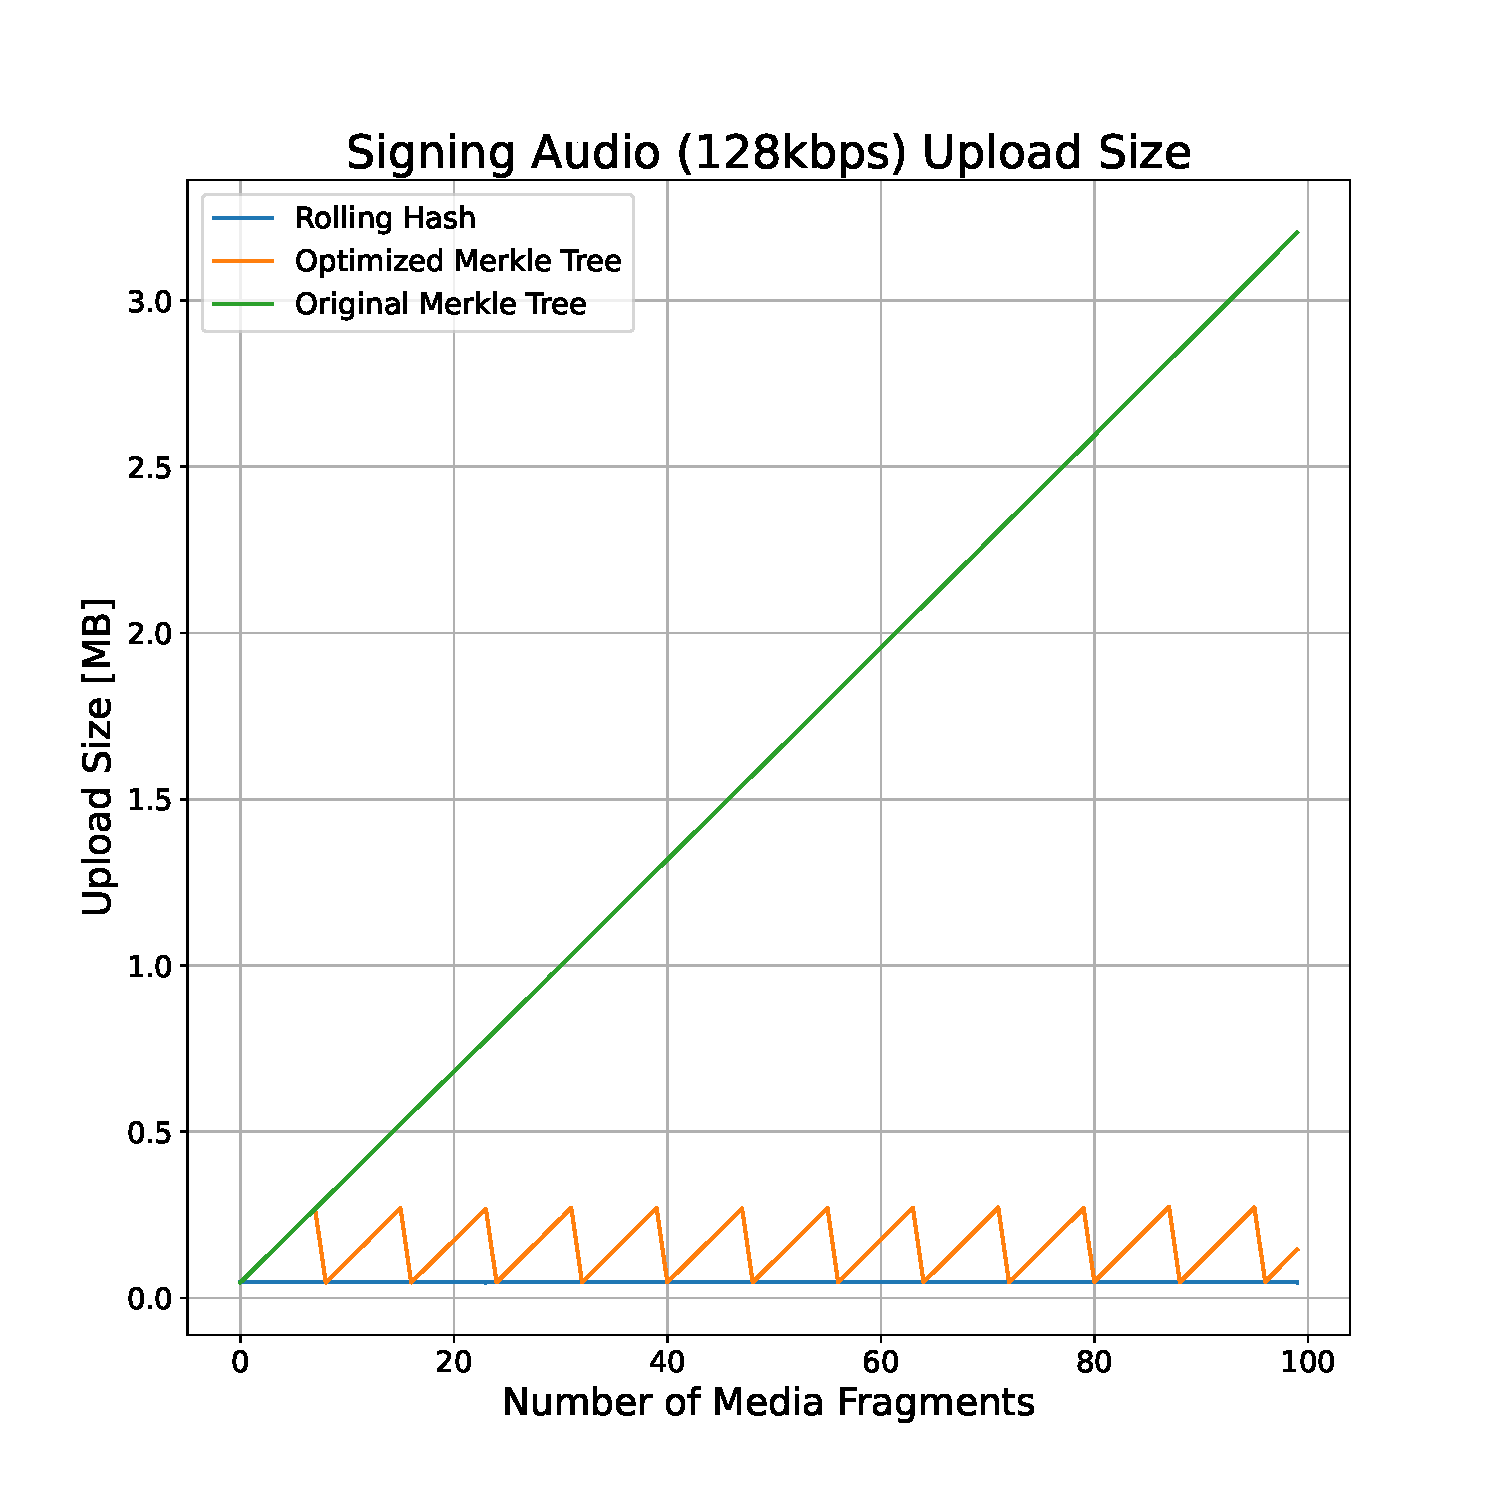
\includegraphics[width=0.49\linewidth]{plots/compare-upload-Audio-(128kbps).pdf}
        \label{fig:upload2-audio}
    }
    \subfloat[Video (276kbps)]{
        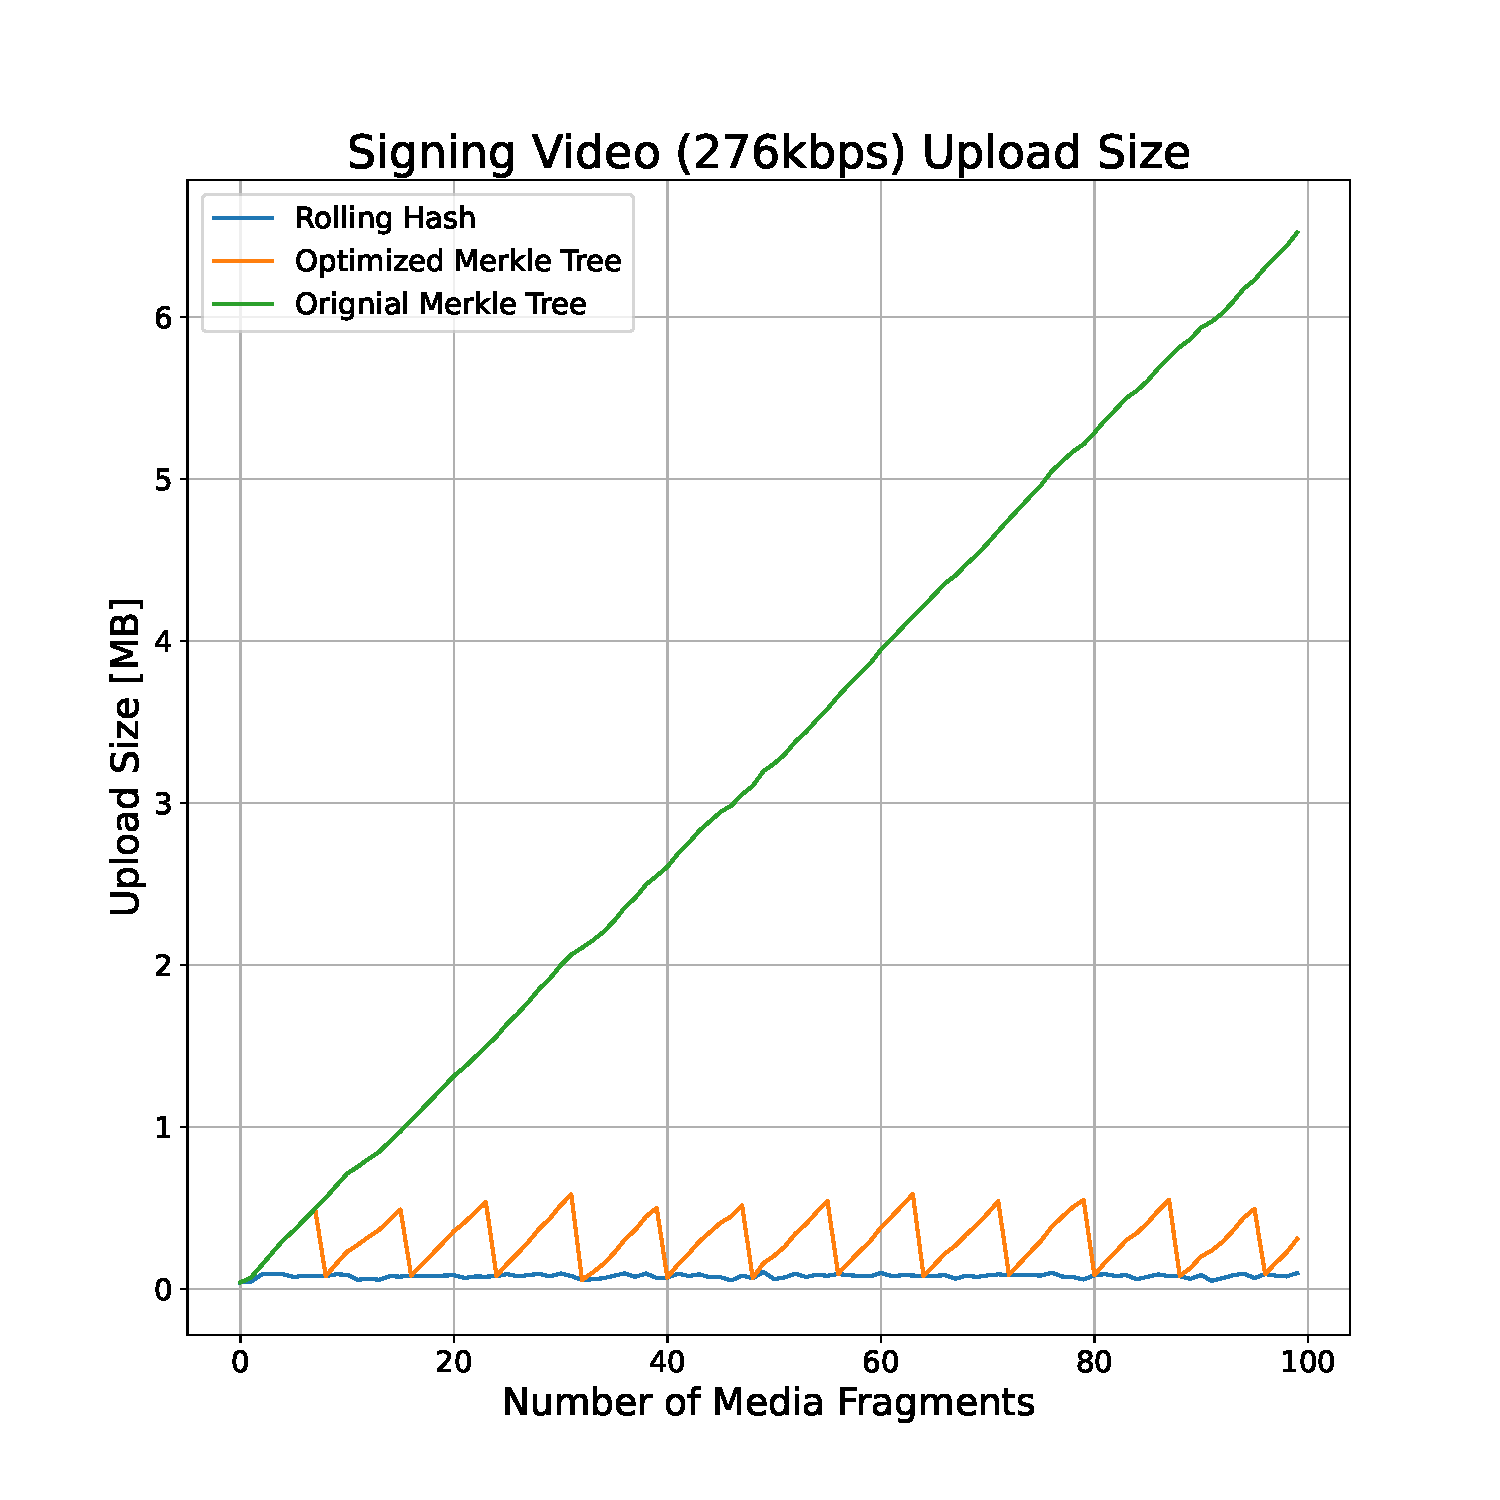
\includegraphics[width=0.49\linewidth]{plots/compare-upload-Video-(276kbps).pdf}
        \label{fig:upload2-video1}
    } \\
    \subfloat[Video (2,048kbps)]{
        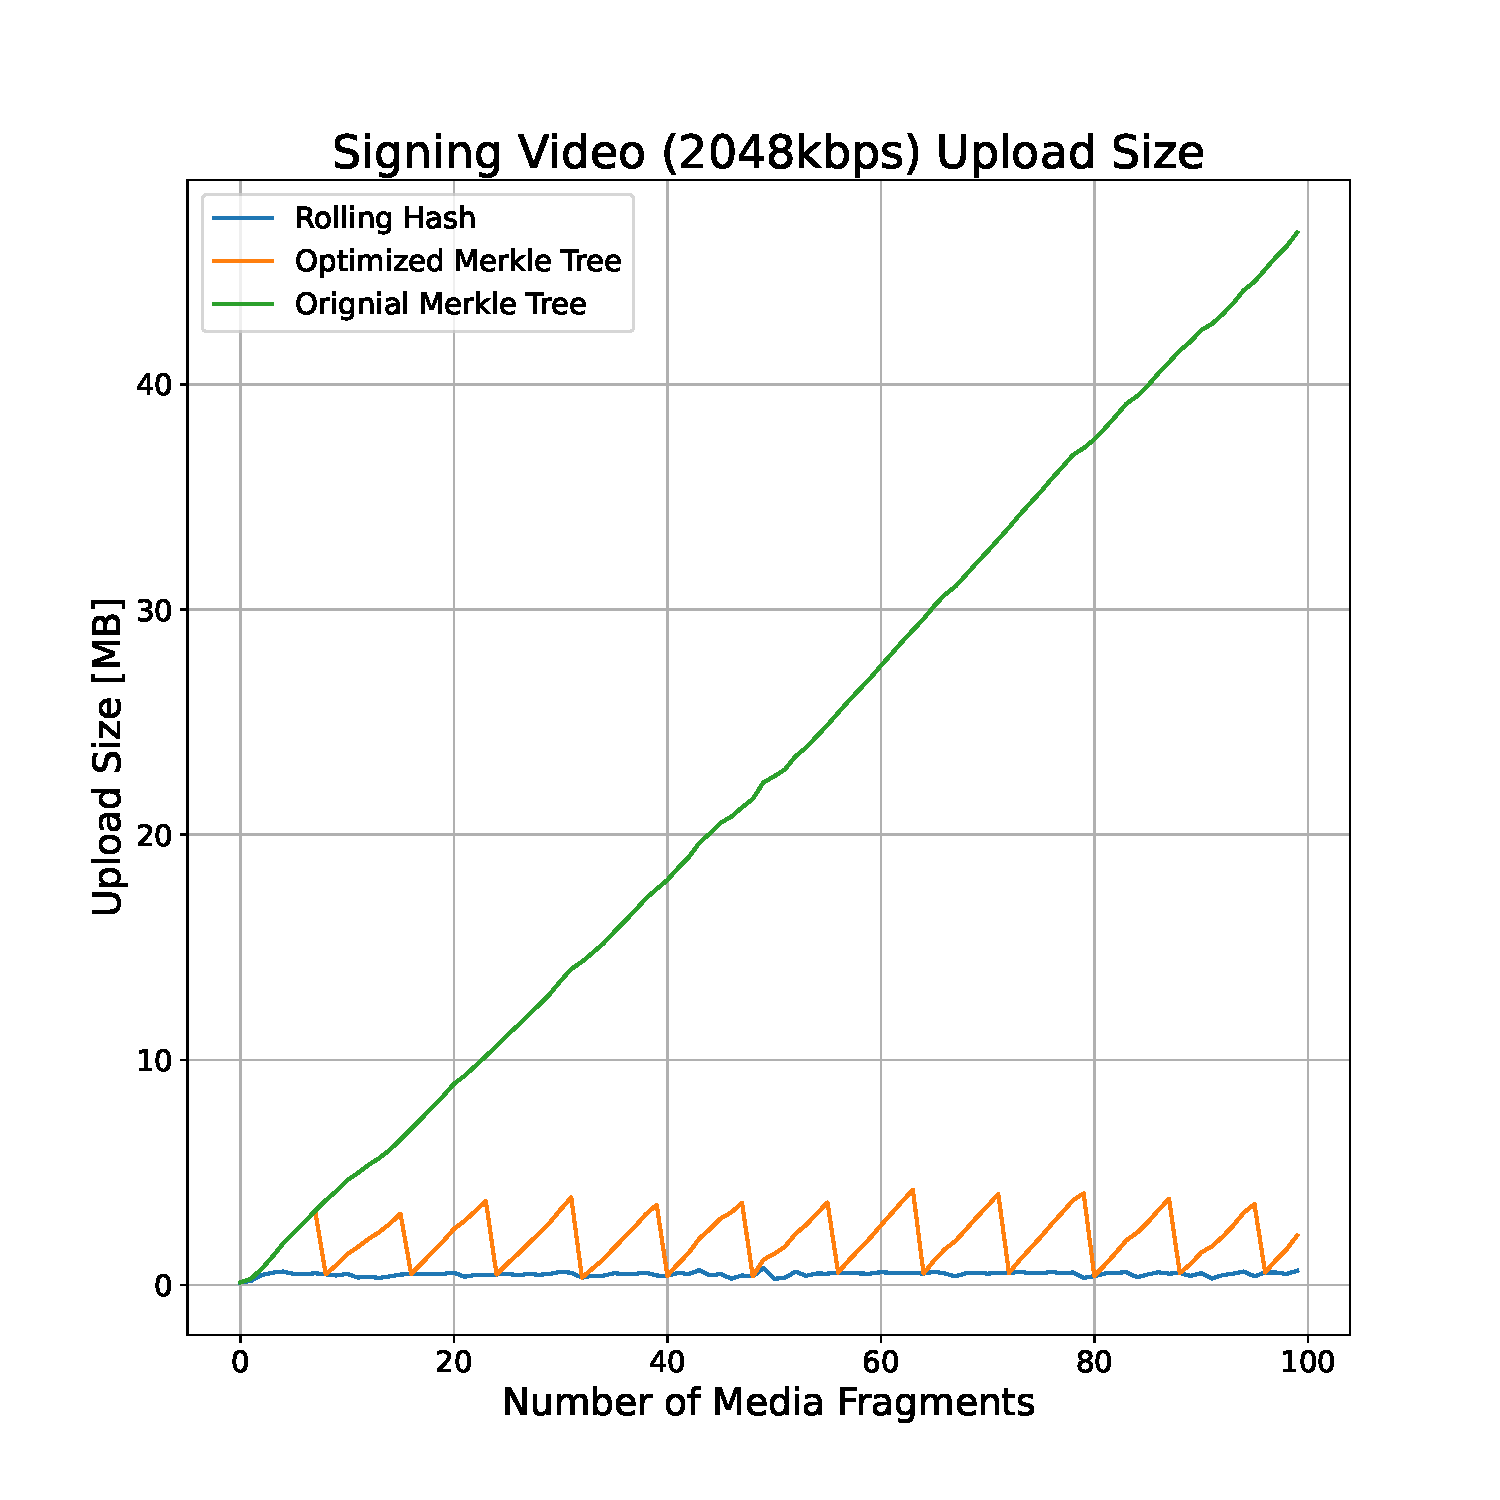
\includegraphics[width=0.49\linewidth]{plots/compare-upload-Video-(2048kbps).pdf}
        \label{fig:upload2-video2}
    }
    \subfloat[Video (17,408kbps)]{
        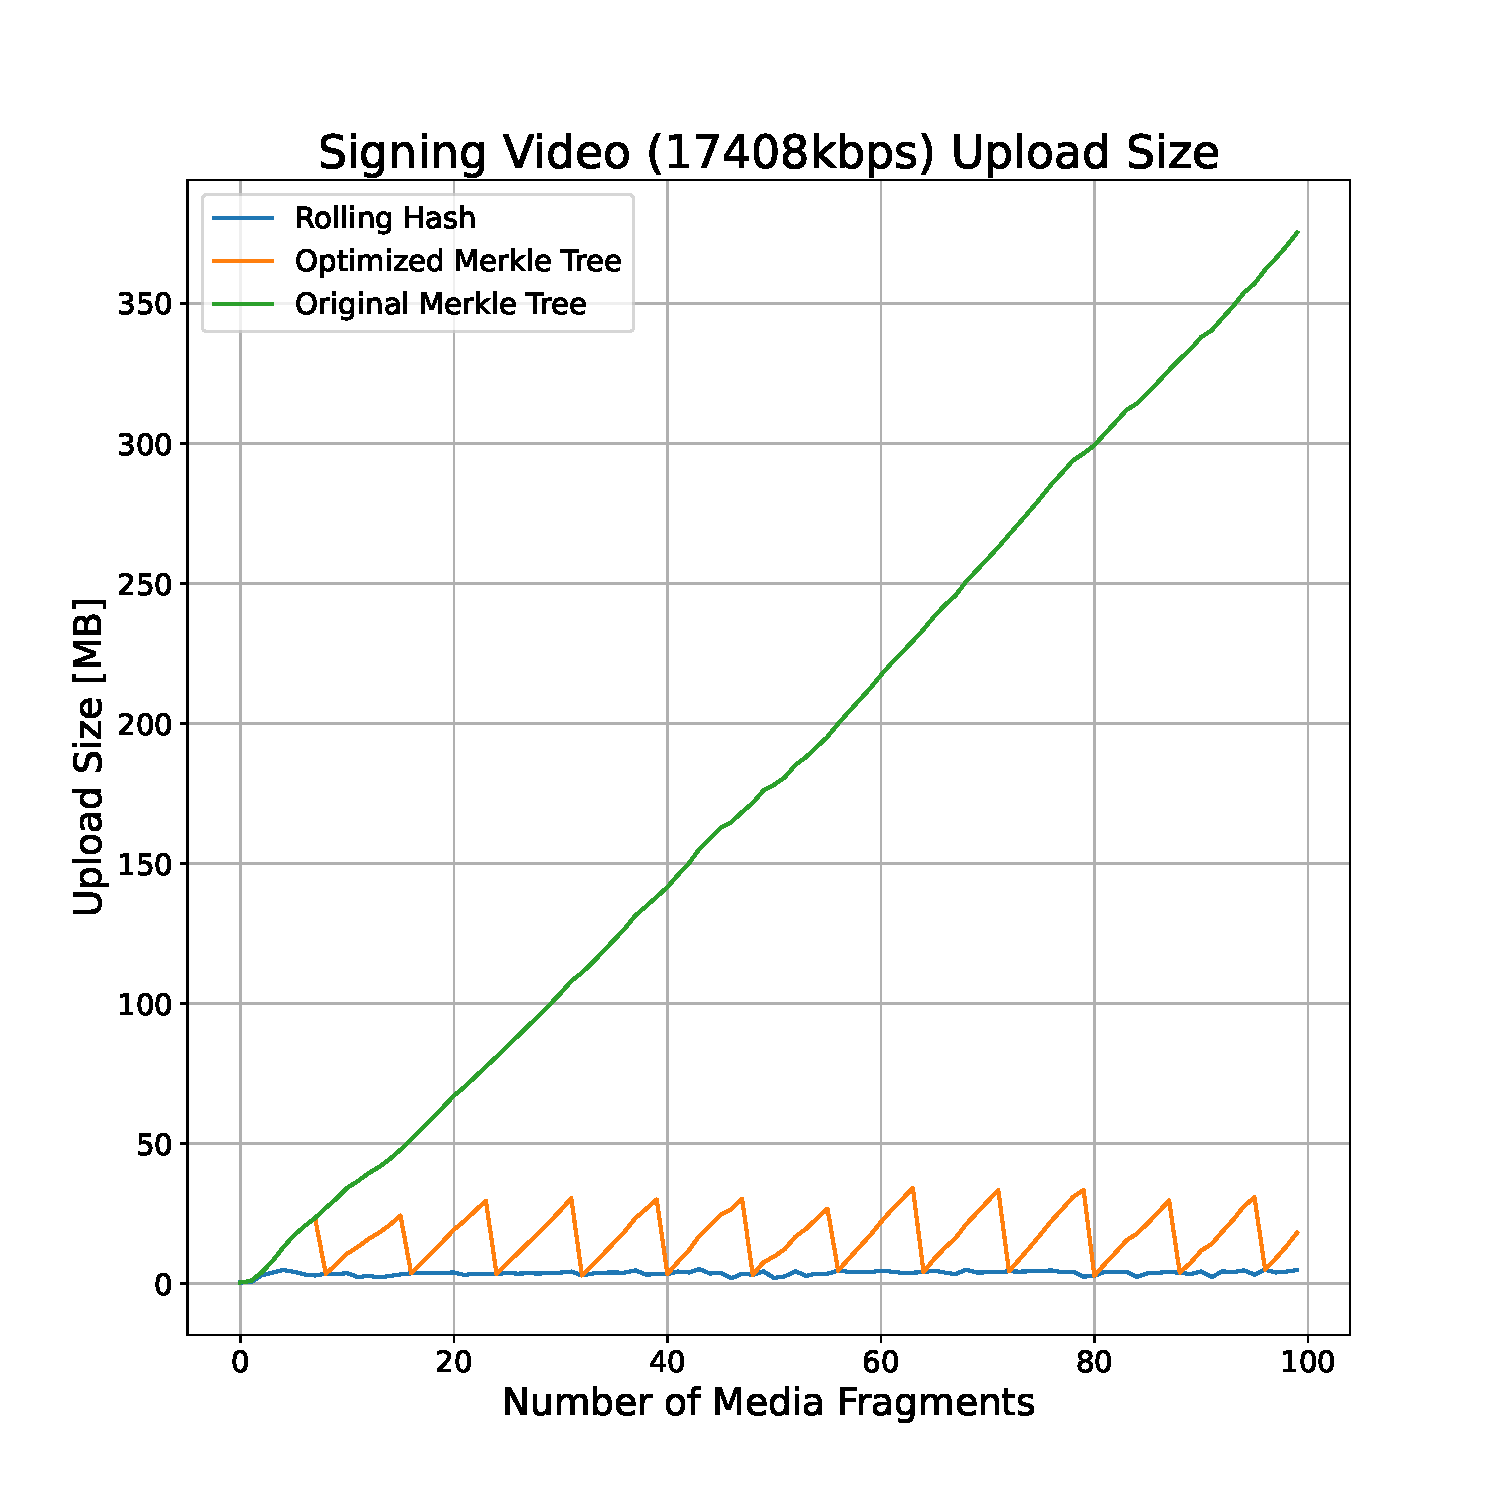
\includegraphics[width=0.49\linewidth]{plots/compare-upload-Video-(17408kbps).pdf}
        \label{fig:upload2-video3}
    }
    \caption{Upload Size Results}
    \label{fig:upload2}
\end{figure}

